\RequirePackage{ifvtex}
\documentclass[12pt,headlines=2,footlines=2,a4paper,twoside,bibliography=totoc]{scrartcl}

\usepackage{ngerman}
\usepackage[utf8]{inputenc}
\usepackage[T1]{fontenc}
\usepackage{setspace}
\usepackage[inner=25mm,outer=40mm,top=25mm,bottom=35mm]{geometry}
\usepackage[font=small,format=plain,labelfont=bf,up,textfont=it,up]{caption}
\usepackage[headsepline,footsepline]{scrlayer-scrpage}
\usepackage{graphicx}
\usepackage{tikz}
\usepackage{hyperref}
\usepackage{float}
\usepackage{longtable}
\usepackage[numbers]{natbib}
\usepackage{soul}
\usepackage{dialogue}
\usepackage{attrib}
\usepackage{pdfpages}

\setcounter{LTchunksize}{100}

\usetikzlibrary{shapes,arrows}

\pagestyle{scrheadings}
\ihead{\headmark}
\ohead{Martin Spoo}
\ifoot{Philosophische Vorstellungen von Kindern zum Thema \glqq Glück\grqq{} in der Grundschule am Beispiel der Grundschule Kesselheim}
\cfoot{}
\ofoot{\pagemark}
\addtolength{\headsep}{0mm}
\addtolength{\footskip}{-5mm}

\bibliographystyle{plainde}

\renewcommand{\figurename}{Abb.}

\begin{document}

%% Titelseite
\thispagestyle{empty}
\newgeometry{inner=1.5cm,outer=1.5cm,head=1.5cm,bottom=1.5cm}
\begin{titlepage}
	\subpdfbookmark{Titel}{pdf:title}
	\begin{center}
		\quad
		\vfill
		\Huge{
			\setstretch{2} \textbf{Philosophische Vorstellungen von Kindern zum Thema \glqq Glück\grqq}
		}
		\vspace{5mm}
		\vfill
		\large{
			{\bfseries Masterarbeit\\
			\vspace{5mm}
			\normalfont \rmfamily zur Erlangung des akademischen Grades\\
			\bfseries Master of Education (M. Ed.)\\
			\vspace{5mm}
			\normalfont \rmfamily im Studiengang Grundschulbildung}
		}
		\\
		\vspace{1.5cm}
		\large{
			{vorgelegt von\\
			Martin Spoo\\
			Matrikelnr.\,212100872}
		}
		\vspace{1cm}
		\\
		\Large{
			{Universität Koblenz-Landau}\\
			{SS\, 2016}
		}
		\vspace{1cm}
		\begin{table}[b]
			\begin{center}
				\begin{tabular}{lr}
					Prüfer: &  Prof. Dr. Heike de Boer , \\
								&	Institut für Grundschulbildung, Campus Koblenz \\
					Zweitprüfer: & Dr. Nicole Henrich \\
					\vspace{0.25cm} \\
					Abgabetermin: & 24. August 2016 \\
					Datum: & \today
				\end{tabular}
			\end{center}
		\end{table}
	\end{center}
\end{titlepage}
\renewcommand{\baselinestretch}{1.1}
\restoregeometry



%% Eine leere Seite nach dem Titelblatt einfügen
\newpage

%% Seitenzähler nach dem Titelblatt auf 1 setzen
\setcounter{page}{1}

%% Inhaltsverzeichnis
\currentpdfbookmark{Inhaltsverzeichnis}{pdf:toc}
\tableofcontents
\newpage

%% Zeilenabstand auf 1,5fach
\onehalfspacing

%% Einleitung
\section{Einleitung}
In der folgenden Hausarbeit soll ein synoptischer Vergleich der biblischen Textstelle Mk 15,38-41 durchgeführt werden. Dabei liegt das besonderere Augenmerk auf der Untersuchung der Evangelien auf inhaltliche und sprachliche Differenzen. Um einen Einstieg zu ermöglichen, will ich die Methode des synoptischen Vergleiches kurz erläutern.
Beim synoptischen Vergleich handelt es sich um eine Untersuchungsmethode, bei der vergleichbare Textpassagen der synoptischen Evangelien tabellarisch nebeneinander gestellt werden. In dieser Hausarbeit wird es sich dabei um die zu Beginn genannte Passage des Markusevangeliums sowie Lk 23,45-49 und Mt 27,51-56 handeln.
Der synoptische Vergleich bietet uns die Möglichkeit, eine Textstelle aus den synoptischen Evangelien nach Markus, Lukas und Matthäus näher zu untersuchen. Nach der Zweiquellentheorie geht man davon aus, dass das Markusevangelium als erstes entstand und als Vorlage für Matthäus und Lukas diente. Diese haben sich wiederum zusätzlich noch einer Logienquelle Q und ihres jeweiligen Sondergutes bedient.
Als Forschungsfrage leitet sich daher ab: „Inwiefern kann man die Zweiquellentheorie anhand der Textpassage Mk 15,38-41 bestätigen?“
Die Wahl des Themas der Passion für einen synoptischen Vergleich ergab sich daraus, dass mir die Passion bereits aus dem Religionsunterricht bekannt ist  und sie zu einem der Themen der Bibel gehört, die mich am meisten interessieren. Da die Größe der Textstelle auf vier Verse vorgegeben war, musste eine Stelle gewählt werden, die inhaltlich und sprachlich genug Untersuchungspunkte bietet. Des Weiteren lässt sich anhand der Leidensgeschichte Jesu gut darstellen, worauf die Evangelisten den inhaltlichen Schwerpunkt in ihren Evangelien legten, um ihre jeweiligen Zielgruppen anzusprechen. 
\newpage

%% Philosophieren in der Grundschule
\section{Philosophieren mit Kindern}

Das Philosophieren ist mittlerweile vor allem an den weiterführenden Schulen im deutschen Bildungssystem angekommen.
 In vielen Fällen wird es sogar als eigenständiges Unterrichtsfach angeboten. 
 Doch auch in der Grundschule gewinnt das Philosophieren mit Kindern stetig an Bedeutung, weshalb es von zentraler Bedeutung ist, zu klären, inwiefern es auch im Sachunterricht der 
 Grundschule Sinn macht, den Schülerinnen und Schülern ein solches Unterrichtsangebot zu machen. 
 
Zunächst soll der Fokus jedoch auf der Betrachtung des Philosophiebegriffs liegen und darauf, was man letztlich tut, wenn man philosophiert.



\subsection{Was versteht man unter Philosophie und Philosophieren?}

Der Begriff \glqq Philosophie\grqq{} setzt sich aus den beiden Ausdrücken \glqq philos\grqq{}, welcher Liebe bedeutet und \glqq sophia\grqq{}, was mit Weisheit übersetzt werden kann, zusammen\cite[S.\,8]{BB10}. 
An anderer Stelle, wie in \cite{GT16}, wird der Begriff \glqq philos\grqq{} hingegen als \glqq Freund\grqq{} übersetzt. 
Von der Wortherkunft lässt sich daher sagen, dass sich die Philosophie als \glqq Liebe zur Weisheit\grqq{} oder \glqq Freundschaft zur Weisheit\grqq{} übersetzen lässt. 

Aufgabe der Philosophen als Philosophie betreibende Menschen und der Philosophie allgemein ist es, \glqq über wichtige Lebensfragen\grqq{} des Menschen und seiner Umwelt nachzudenken\cite[S.\,8]{BB10}. 

Brüning beschreibt, dass sich zwei zentrale Formen der Philosophie entwickelt haben. 
Die esoterische Philosophie beruht darauf, dass seit den Anfängen der griechischen Philosophietradition ein weitreichendes Wissen über die Welt und ihr Dasein gesammelt und zusammengetragen wurde. 
Dieses Wissen wurde dann an philosophischen Hochschulen und Universitäten gelehrt und in eine akademische Disziplin überführt, welche sich folglich Philosophie nennt. 
Darüber hinaus wird in der esoterischen Philosophie angenommen, dass lediglich diejenigen Menschen auch Philosophen sein können, die sich beruflich und mit der Absicht der Forschung mit den Fragen über die Welt beschäftigen.

Demgegenüber steht die exoterische Philosophie, welche ein entgegengesetztes Bild der Philosophie als Disziplin als gegeben ansieht. 
Demnach sind im Wesentlichen alle Menschen in der Lage, sich über die zentralen philosophischen Themen Gedanken zu machen. 
Dabei ist es unerheblich, ob dies aus persönlicher Neugierde oder aus dem Bedürfnis nach Forschungszuwachs geschieht. 
Ferner ist für die exoterische Philosophie auch nicht von Bedeutung, ob das Nachdenken über Philosophisches in einer regelmäßigen Auseinandersetzung stattfindet oder ob der Anspruch des Philosophen erhoben wird, haltbare Theorien zu entwickeln\cite[S.\,8]{BB10}.

Dr. Holm Bräuer, der an der TU Dresden im Institut für Philosophie tätig ist, bezeichnet die Philosophie als wissenschaftliche Disziplin, welche im Gegensatz zu anderen Einzelwissenschaften vor allem gemeingültige Fragen behandelt.
 Dabei sieht auch er vor allem die Frage nach dem Wesen der Welt, aber auch nach dem Sinn des Lebens oder den Ursachen für \glqq Vergangenes und Zukünftiges von religiösen oder mythischen Lehren und Legenden oder von Weltanschauungen\grqq{} \cite{PL16} als zentrale Fragen der Philosophie an.

 Ziel der Philosophie ist es dabei aus seiner Sicht, auf diese allgemein gefassten Fragen der Menschheit Erklärungen zu finden, welche auf der Basis von rationalen Zusammenhängen zustande kommen.
  Bräuer bezieht sich insbesondere auf die Grundfragen Immanuel Kants, der die philosophischen Probleme mit vier Fragen erstmals resümierte: \glqq Was ist der Mensch?\grqq{}, \glqq Was kann ich wissen?\grqq{}, \glqq Was soll ich tun?\grqq{}, \glqq Was darf ich hoffen?\grqq{}.  
  
Im Laufe der Geschichte hat sich die Philosophie durch die verschiedenartigen Fragen, mit denen sie sich beschäftigt, in Teildisziplinen untergliedert, die sich unter den Bereichen der Metaphysik, der Physik und der Ethik fassen lassen. 
Über diesen drei Teildisziplinen stehen einerseits die theoretische Philosophie, die sich vor allem auf den Erkenntnisgewinn und das Verstehen der Welt konzentriert, andererseits die praktische Philosophie, die die Aufmerksamkeit vor allem auf das Handeln des Menschen aus philosophischer Sichtweise richtet. 
Die Teilbereiche der Metaphysik und der Physik lassen sich der theoretischen Philosophie, die Ethik und dabei vor allem die Staatsphilosophie und die Rechtsphilosophie der praktischen Philosophie zuordnen. 

Die Tätigkeit des Philosophierens sieht Barbara Brüning vor allem durch einen Aufbau gekennzeichnet, der sich anhand von zentralen Merkmalen manifestiert. 
Am Beginn eines jeden Philosophierens sieht sie zunächst das Staunen, das dazu führt, das etwas zuvor als trivial Angesehenes von nun an kritisch hinterfragt wird und nach Begründungen für Existierendes gesucht wird. 
Aus diesem Staunen entspringt in einem weiteren Schritt das Fragen. 
Der Mensch möchte erfahren, warum sich Dinge verhalten, wie sie es tun und gehen damit \glqq erste Schritte auf dem Weg zu neuen Erkenntnissen\grqq{} \cite[S.\,10]{BB10}. 
Interessant ist an dieser Stelle auch die Erkenntnis John Lockes, auf den sich Brüning bezieht, der feststellte, dass bereits Kinder Fragen nach dem Wesen der Welt stellen würden. 
Daher empfiehlt Locke den Eltern grundsätzlich, den Drang der Kinder nach Wissen zu erhalten und durch Antworten, welche neue Fragen hervorrufen, weiterzuführen.

Die Fragen die sich der Mensch stellt, möchte er in der Folge selbstverständlich auch beantwortet wissen. 
Daher liegt der nachfolgende Schritt im Nachdenken, welches sowohl im Nachdenken des Einzelnen, aber auch im Diskurs mit Anderen vollzogen werden kann. 

Das Nachdenken vollzieht sich nach Brüning in einem Dreischritt. 
Zunächst müssen im philosophischen Diskurs Begriffe ge-- bzw. erklärt werden, um sich dem zentralen Gegenstand der jeweiligen Frage nähern zu können. 
Tauscht man sich beispielshalber über die Frage aus, ob es ein Leben nach dem Tod gibt, so muss zunächst geklärt werden, was das Leben eines Lebewesens ausmacht und was der Tod bedeutet. 
Somit wird zunächst eine Standortbestimmung der Begrifflichkeiten vorgenommen. 
Anschließend werden Gründe dafür gesucht, die eine Position bejahen oder verneinen können und darüber geurteilt, welche Argumente am stichhaltigsten sind, um eine Sicht zu untermauern. 
Im sokratischen Gespräch können solche Begründungen dann kontrovers diskutiert und dabei bestätigt oder widerlegt werden. 
Dabei muss das Gespräch keine feste Lösung ergeben, sondern es können auch sich ausschließende Antworten Seite an Seite stehen bleiben\cite[S.\,11]{BB10}.

Das Philosophieren kann und möchte trotz rational begründeter Annahmen nicht den Anspruch erheben, vollständig beweisbare Antworten zu liefern. 
Das hat zur Folge, dass jede philosophische Antwort Zweifler finden wird, die Gegenargumente heranziehen werden. 
Daher gehört zum Philosophieren auch die Erkenntnis, zu wissen, dass solche Antworten stets nur einen Teil der Realität abbilden und daher nur provisorischen Charakter haben können. 
Dazu gehört auch, dass bei jeder Diskussion auch die gänzlich gegensätzliche Ansicht als denkbar anerkannt werden muss. 
Die Erkenntnis darüber und die Zweifel an der Antwort auf eine Frage bringen es mit sich, dass die Gedanken des Zweifels weitergedacht werden müssen. 
Dadurch wird der Prozess des Überlegens am Leben erhalten und das Weiterdenken, wie Brüning es nennt, kommt zustande. 
Den Abschluss des Weiterdenkens bringt dann die Einsicht, \glqq dass der Prozess des Nachdenkens über ein philosophisches Problem unabgeschlossen bleibt\grqq{} \cite[S.\,13]{BB10} und es eine \glqq richtige\grqq{} Antwort nicht geben kann.

Am Schluss des Philosophierens wird das eigene Denken infrage gestellt, angezweifelt und unter Umständen auch korrigiert. 
Wird die gleiche Thematik erneut diskutiert, ist es demnach möglich, dass eine zuvor als korrekt angesehene Antwort inzwischen überarbeitet oder gänzlich neu gefasst wurde. 
Daher sieht es Barbara Brüning als besonders zentral an, im Philosophieren mit Kindern in der Grundschule die Antworten der Kinder stets dahingehend zu hinterfragen, ob auch die andere Sichtweise für möglich erachtet wird.


\newpage
\subsection{Eigenschaften philosophischer Unterrichtsgespräche}

Allgemein versteht man unter Unterrichtsgesprächen Gespräche, die im schulischen Kontext -- vor allem im Unterricht zwischen Lehrern und Schülern -- geführt werden. 
Im Gegensatz zu Alltagsgesprächen zwischen Fremden oder der Unterhaltung im familiären Rahmen sind diese Gespräche \glqq institutionell geprägt\grqq{} \cite[S.\,28]{HB15}. 
Daher folgen sie auch schulisch geprägten Normen und die verwendete Sprache ist eine auf diesen Kontext zugeschnittene. 
Feilke fand dazu heraus, dass \glqq die Schulsprache keine Bildungssprache sei, sondern ein Instrument der Erziehung zur Bildungssprache; denn ein kompetenter Sprachgebrauch werde orientiert an den Vorstellungen der Schule und Schulfächer aufgebaut.\grqq{} \cite[S.\,117]{HF13}

De Boer verweist auf Lüders, der davon ausgeht, dass sich das Unterrichtsgespräch in ein wiederkehrendes Muster einordnen lässt\cite[S.\,28]{HB15}:
 Zunächst geht von der Lehrperson eine \textit{initiation}, beispielsweise eine Frage, aus, auf die Schüler meistens mit einem \textit{reply} bzw. einer Antwort reagieren. 
 Schließlich wird die gegebene Antwort in der \textit{evaluation} hinterfragt und der Prozess beginnt erneut. 
 Es lässt sich daher sagen, dass in einem klassischen Unterrichtsgespräch immer eine Validierung vorgenommen wird, die sich bei Lüders in der \textit{evaluation} finden lässt. 
 Für das philosophische Unterrichtsgespräch ist jedoch zu sagen, dass es vor allem gilt, \glqq dem gemeinsamen Nachdenken Raum zu geben, unterschiedliche Denkwege auszutauschen, Fragen zu entwickeln und ein offenes Gespräch ohne Validierungszwänge zuzulassen\grqq{} \cite[S.\,159]{HD15}.
 
Das Unterrichtsgespräch befindet sich darüber hinaus in zwei zentralen Spannungsfeldern. 
Zum einen muss die Lehrkraft eine Organisation vornehmen, die für die Schüler einerseits durch den gewählten Zeitpunkt und andererseits durch Transparenz im Umgang Klarheit vermittelt, zum anderen führt eine detaillierte Planung zu repetierenden Abläufen\cite[S.\,31]{HB15}. 
Das zweite Spannungsfeld sieht die Lehrperson vor dem Problem, das Gespräch fachlich fundiert zu führen und darüber hinaus auch flexibel zu gestalten, um auf situationsbedingte Veränderungen reagieren zu können. 
Daher wird von den Lehrerinnen und Lehrern eine zunehmend selbstreflektierte Moderatorentätigkeit verlangt.

Ziel des philosophischen Gesprächs sollte es sein, einen Dialog zwischen den Schülerinnen und Schülern herzustellen. 
Martin Buber entwickelte dazu drei Merkmale, die für ihn ein dialogisches Gespräch ausmachen. 
Zum einen müssten sich die Gesprächspartner einander zuwenden, d.h. die Existenz des Anderen akzeptieren und nicht seine Gedanken und Handlungen widerspruchslos  übernehmen\cite[S.\,106]{MB15}.
Weiter erachtet es Buber für wichtig, dass die Gesprächspartner eigene Gedanken einbringen und diese unverkürzt wie uneingeschränkt zur Sprache bringen. 
Zuletzt sollte in einem Dialog auf die Selbstdarstellung verzichtet werden, da dann nicht die eigentlichen Positionen mitgeteilt werden, sondern die authentische Komponente des Gesprächs verloren geht.

Für philosophische Unterrichtsgespräche ergeben sich in Bezug auf die dialogische Ausgestaltung zusätzliche Merkmale, die nicht vernachlässigt werden dürfen. 
Grundlegend ist zu philosophischen Unterrichtsgesprächen zu sagen, dass es sich bei ihnen um sokratische Gespräche handelt. 
Diese Gesprächsform zeichnet sich vor allem dadurch aus, \glqq dass in ihm ein philosophischer Gegenstand diskutiert wird, bspw. Glück, Gerechtigkeit oder Freundschaft.\grqq{} \cite[S.\,27]{BB10}

Ein sokratisches Gespräch, wie es auch mit Schülern in der Grundschule geführt werden kann, gliedert sich in drei Phasen. 

In der ersten Phase, welche Brüning Vorbereitungsphase nennt, geht es vor allem darum, die zentrale philosophische Fragestellung zu klären. 
Dabei kann die Fragestellung sowohl die eines Kindes als auch die der Lehrperson sein. 
Daneben müssen Regeln für den Ablauf des Gespräches aufgestellt werden, welche im gesamten Gesprächsverlauf eingehalten werden müssen. 
Dazu können das aktive Zuhören, das Begründen der eigenen Meinung gehören aber auch, andere ausreden zu lassen\cite[S.\,31]{BB10}.
In der zweiten Phase kommt es zum eigentlichen philosophischen Gespräch. 
Das zuvor ausgewählte Thema wird mit den Schülerinnen und Schülern diskutiert und die Lehrerin bzw. der Lehrer übernehmen lediglich die Aufgabe des Moderators. 
Brüning weist ausdrücklich darauf hin, dass auch ein Schüler diese Tätigkeit wahrnehmen kann, wenn die Schülerinnen und Schüler bereits mit dem gemeinsamen Philosophieren vertraut sind. 
Während des Gespräches sollen auch unbekannte Begriffe geklärt und über die Thematik argumentativ gestritten werden. 
Gegen Ende des Gespräches soll sich dann ein gemeinsames Ergebnis herauskristallisieren. 
Dieses kann entweder in einer alleinigen Lösung oder aber in verschiedenen bestehen. 

An diese Phase schließt sich in einem dritten Schritt das Metagespräch an, in  dem das gemeinsame Nachdenken unterbrochen wird oder ein Anschluss an die Diskussion gefunden wird. 
Unter anderem beschreibt Brüning, dass in diesem Teil des sokratischen Gespräches die Einhaltung der Regeln erneut diskutiert und auf etwaige Verletzungen hingewiesen werden kann. 
Zudem können die Ergebnisse des Gespräches an dieser Stelle erneut zusammengefasst werden.

Während für ein Unterrichtsgespräch generell vor allem der gedankliche Lernprozess des Kollektivs im Vordergrund steht, ist dies allein für das philosophische Gespräch nicht mehr ausreichend. 
Vielmehr muss den Schülerinnen und Schülern näher gebracht werden, die Sichtweisen und Blickwinkel anderer zu verstehen und akzeptieren zu können\cite[S.\,234]{HDB15}. 
Auch muss für philosophische Unterrichtsgespräche das Rollenbild zwischen Lehrperson und den Schülerinnen und Schülern aufgebrochen werden. 
Bleibt es nämlich, wie bei dieser Gesprächsform üblich, dabei, dass ausschließlich die Lehrerin bzw. der Lehrer die Fragen stellt, werden die Schüler nicht in der Art und Weise für die Thematik zu begeistern sein, wie in dem Falle, in dem sie selbst ihre Fragen in den Raum stellen dürfen. 
Daher würde bei einer klassischen Anordnung im philosophischen Gespräch die Chance, Lernprozesse bei den Schülerinnen und Schülern zu initiieren, verpuffen.

Für de Boer wird das Philosophieren mit Kindern dann zum Unterrichtsprinzip, wenn Lehrerinnen bzw. Lehrer und Erwachsene im Allgemeinen dazu beitragen, dass das kategoriale Denken der Kinder in weitergehende und multidimensionale Denkweisen übertragen werden.


\newpage
\subsection{Warum sollte in der Grundschule philosophiert werden?}

In den letzten Jahren hat sich der pädagogische Blick auf das Philosophieren an Schulen kontinuierlich gewandelt. 
So wurden teilweise von Philosophen selbst Gesprächsanlässe und Konzeptionen geschaffen, die die Schülerinnen und Schüler als selbständige Menschen sehen und ihnen die Möglichkeit geben wollen, sich die Welt autonom zu erschließen\cite[S.\,617]{AN13}. 
In diesem Kontext wurde auch die Frage diskutiert, ob das Philosophieren mit Kindern als eigenes Unterrichtsfach angeboten oder in bereits vorhandenen Fachunterricht eingebettet werden soll. 

Professor Dr. Andreas Nießeler, der an der Universität Würzburg in den Bereichen Grundschulpädagogik und Theorie des Sachunterrichts, Philosophieren mit Kindern, Kulturanthropologische Theorie der Bildung und des Lernens und Bildungsphilosophie und pädagogische Anthropologie forscht und lehrt, stellt klar, dass das Ziel des Philosophierens mit Kindern aus pädagogischer Sicht vor allem darin besteht, \glqq junge Menschen mit ihren Fragen ernst zu nehmen\grqq{} \cite[S.\,617]{AN13}.
Hinzu kommt, dass die Schülerinnen und Schüler in die Lage versetzt werden sollen, ihre Deutung von der Welt ausdrücken zu können und sich eigenständig in ihrem Denken zu orientieren. 

Nießeler erwähnt dazu Herman Nohl, der in seiner 1922 veröffentlichten Schrift \glqq Philosophie in der Schule\grqq{} feststellt, dass der Philosophieunterricht \glqq anstatt als Einzelfach ein trauriges Dasein zu fristen die Gesamtheit der Fächer zu tragen habe und dessen Aufgabe eine Erziehung zur \glqq Vergeistigung unseres Seins, Denkens und Tuns durch Rückbeziehung alles Einzelnen auf Sinn und Grund, eine platonische Anleitung zur Erhebung in das höhere geistige Leben der Idee\grqq{} sei.\grqq{} \cite[S.\,618]{AN13}
Hier zeigt sich die Verortung der Philosophie in der Schule, die keinen eigenen Platz in der Fächerlandschaft der Grundschule zugewiesen bekommt und deren Ziel es ist, ein autonomes Denken unter den Schülerinnen und Schülern zu etablieren. 
Darüber hinaus spricht Andreas Nießeler die Ideen des Philosophen Leonard Nelson an, der als zentrale Unterrichtsmethode die sokratische Maieutik betrachtete. 

Diese Methode, auch Hebammenprinzip, sah nach Sokrates vor, durch gezielte Fragen das vorhandene Wissen des Befragten zutage zu fördern. 
Mithilfe dieser Maieutik wollte Nelson den Schülern die Unvollständigkeit des Wissens deutlich machen. 
Hauptsächlich ging es ihm darum, dass die Schülerinnen und Schüler nicht lernen sollten, was Philosophie ist, sondern sie sollten das Philosophieren als solches lernen und so selbst zu Philosophen werden\cite[S.\,618]{AN13}. 

Ferner bezieht sich Nießeler darauf, dass die ersten, wissenschaftlichen Untersuchungen vor allem in den USA stattfanden. 
Matthew Lipman, der 1974 das \glqq Institute for the Advancement of Philosophy for Children\grqq gründete, war zusammen mit Gareth B. Matthews einer der ersten, die ein Philosophiekonzept für die Durchführung mit Kindern entwickelten. 
Lipman war der überzeugung, dass Kinder bereits früh in der Lage sind, logisch zu denken und sah das logische Denken daher als eine Basisqualifikation an\cite[S.\,619]{AN13}. 
Matthews hingegen untersuchte vor allem philosophische Gespräche zu verschiedenen Themen wie \glqq Glück\grqq{}, \glqq Wünsche\grqq{} oder \glqq Gerechtigkeit\grqq{}. 
Er konnte durch Erinnerungsprotokolle ermitteln, dass in diesen Gesprächen bei den Kindern eine Entwicklung stattfindet und philosophische Gespräche es erlauben, die philosophischen Vorstellungen von Kindern in Relation zu bedeutenden Fragen untersuchen zu können.

Barbara Weber stellt in ihrem Beitrag \glqq Philosophieren mit Kindern: Wieso, Weshalb, Wozu?\grqq{} fest, dass das Philosophieren mit Kindern einerseits aus pädagogischer andererseits aus philosophischer Sicht in der Kritik stehe. 
Es werde argumentiert, man könne die Schülerinnen und Schüler überfordern, wenn man mit ihnen philosophische Themen erörtert, andererseits ist die Bedeutung der Philosophie in sich eine der größten Fragen, der sich die Philosophie entgegensieht. 
Weber hebt hervor, dass es Skeptiker gebe, die den Kindern nicht die Fähigkeiten zusprechen würden, sich ein umfassendes Wissen über philosophische Themen anzueignen, aber auch Befürworter, die in der Philosophie eine umfassende pädagogische Lösung sehen würden, mit deren Hilfe jegliche sozialen und inhaltlichen Kompetenzen erworben werden könnten\cite[S.\,623]{BW13}.
Jedoch sollten überhöhte Erwartungen an das Philosophieren mit Kindern vermieden werden. 

Entscheidend sei aus ihrer Sicht auch, welche Themen für das Philosophieren gewählt würden und ob diese philosophisch gesichert seien, was Ekkehard Martens 1999 bezweifelt habe\cite[S.\,624]{BW13}. 
Das Philosophieren in Unterrichtsgesprächen mit Kindern kann für Barbara Weber von großem Nutzen für die pädagogische Forschung sein. 
Nutzt man es als qualitative Methode, so könne man aus diesen Gesprächen Rückschlüsse daraus ziehen, wie Schülerinnen und Schüler über philosophische Themen denken und was sie dazu sagen.

Weber erstellt ein Schema, nach dem sich philosophische Gespräche grob gliedern lassen. 
So geht jedem philosophischen Gespräch ein Staunen und Fragen voraus, in dem die Schülerinnen und Schüler sich über eine Fragestellung klar werden und diese hinterfragen. 
Dem schließt sich der gemeinsame Dialog mit Anderen - das Denken-Sprechen - an, der die Positionen anderer in den Blick nimmt und gegebenenfalls auch die eigenen verändern kann. 
In einem weiteren Schritt kommt es zum Werten-Handeln, das zu einer Prüfung oder sogar Veränderung der eigenen Lebenswelt führen kann. 
Eigenes Handeln und individuelle Werte werden geprüft und dies führt zu weiterem Staunen und Fragen\cite[S.\,626]{BW13}.
Barbara Weber betrachtet das gesammelte Wissen der Philosophie nicht als abgeschlossen, sondern verweist auf Pierre Hadot, der in seinem Werk \glqq Wege zur Weisheit\grqq{} darauf hinwies, dass \glqq die Philosophie ein historisches Phänomen ist, das zu einer Zeit begonnen und sich bis heute weiterentwickelt hat.\grqq{}
Diese Sicht auf die Philosophie hat zur Folge, dass diese nicht mehr bloß Modelle behandelt, sondern sich auch mit philosophischen Verhaltens- und Lebensweisen beschäftigen müsse.

Kerstin Michalik verortet das Philosophieren in einem eigenen Unterrichtsprinzip, dass die Schülerinnen und Schüler in ihren persönlichen Lernprozessen unterstützen und ihnen die Möglichkeit bieten soll, ein differenziertes Weltbild zu entwickeln\cite[S.\,635]{KM13}. 
Weiter schließt Michalik in ihrem Beitrag an die Ausführungen von Andreas Nießeler an, der die Frage nach der Philosophie als eigenständigem Unterrichtsfach aufwarf. 
Sie sieht die Philosophie als Unterrichtsprinzip in den Fachunterricht eingebettet durch philosophische Gespräche mit den Kindern. 
Es geht dabei nicht um die Einführung neuer Inhalte, wie es in den anderen Fächern des Grundschulunterrichts der Fall ist, sondern um überfachliche Zugänge zu Fragen, mit denen sich die Schülerinnen und Schüler auseinander setzen. 
Dadurch eröffnet das Philosophieren mit Kindern vollkommen neue Möglichkeiten im interaktiven Lernen. 
Die Schüler werden durch die Gestaltung des Unterrichts und die Gelegenheit, eigene Fragen in den Unterricht einzubringen, an ihrem Lernstand abgeholt und es wird eine besondere Bedeutsamkeit für sie geschaffen.

Michalik stellt klar, dass Kinderfragen im alltäglichen Unterrichtsgeschehen keine besonders große Wichtigkeit zugeschrieben wird. 
Dem kann das Philosophieren als Unterrichtsprinzip entgegenwirken, indem es diese Fragen zum Ausgangspunkt des Unterrichts macht. 
Sie erörtert, dass der klassische Unterricht vor allem durch Lehrerfragen dominiert wird, die darauf ausgerichtet sind, vorhandenes oder zu erwerbenes Wissen abzufragen und zu festigen. 
Sie haben zudem einen \glqq fixierenden und einschränkenden Charakter\grqq{} \cite[S.\,635]{KM13}. 
Sie stellt jedoch den Stellenwert von Schülerfragen in Bezug auf den Lernprozess der Schülerinnen und Schüler heraus und knüpft an die Positionen des US-amerikanischen Medienwissenschaftlers Neil Postman an, der eine Perspektivenumkehr forderte, infolge derer das Stellen von Fragen als \glqq Kunst und Wissenschaft beizubringen\grqq{} \cite[S.\,636]{KM13} sei. 
Das Stellen von Fragen hängt zusätzlich eng mit dem Bildungsbegriff zusammen. 
So sagt der Philosoph Peter Bieri, dass man sich bilde, um etwas zu werden. 
Dabei gehe die Bildung immer von einer Neugierde und damit von eigenen Fragen aus.
Michalik weist darauf hin, dass es das Ziel des Philosophierens mit Kindern sein müsse, \glqq das Fragenstellen zu ermutigen und zu fördern und den Kindern zu zeigen, dass das gemeinsame Nachdenken über schwierige Fragen interessant und lohnenswert ist.\grqq{} \cite[S.\,637]{KM13}
Sie beschreibt, dass das klassische Unterrichtsgespräch vor allem von einer Lehrerrolle dominiert wird, die über umfassendes Wissen verfügt und Fragen stellt, die das Gespräch zu vorgefertigten Antworten lenken.

Daher müsse nach den Erkenntnissen Rainer Kokemohrs eine Modalisierung und Validierung stattfinden, um das Gespräch in Gang zu halten und offen zu gestalten.
Unter Modalisierung versteht Kokemohr \glqq die Öffnung des Gespräches hin zu konkurrierenden Lesarten.\grqq{} \cite[S.\,637]{KM13}
Das bedeutet, dass den Interpretationen und Denkweisen mehr Raum zugestanden wird.
Die Validierung hingegen bezeichnet die gegensätzliche Vorgehensweise, durch die das Ende eines Gespräches herbeigeführt wird, indem dieser Spielraum immer weiter eingeengt wird.
Die Schule stehe unter einem Validierungszwang, der dazu führe, dass einige mögliche Lern- und Verstehensprozesse verloren gehen würden.
 
Das Philosophieren mit Kindern kann nach Weber dazu beitragen, den Blick auf das Wissen, dass die Schule vermittelt, zu erneuern.
Werde durch die Schule bisher überwiegend Wissen vermittelt, dass sich durch begründbare Tatsachen charakterisiere, so könne das Philosophieren den Kindern zeigen, dass nicht alles in der Welt \glqq restlos vermessen, geordnet und erklärt ist, sondern auch Raum für Staunen, Nachdenklichkeit, Weiterfragen, Forschen bietet.\grqq{} \cite[S.\,639]{KM13}
Die Schülerinnen und Schüler sollten daher auch lernen, dass das Wissen des Menschen keineswegs allumfassend oder abgeschlossen ist, sondern, dass es immer Fragen gebe, die nicht abschließend beantwortet werden könnten.
Daher sei es wichtig, den Kinder diese Erfahrung der Begrenztheit von Wissenschaft zu ermöglichen und so \glqq Grundlagen für ein reflektiertes und differenziertes Welt- und Wissenschaftsbild zu legen.\grqq{} \cite[S.\,640]{KM13}
Für Michalik kann das Philosophieren dazu dienen, dem Lernen der Kinder einen Sinn zu geben und es vom Stigma des bloßen Bewältigens von Arbeitsaufträgen zu lösen.
Sie betont, dass Wissenschaft und Philosophie keine Gegensätze seien, sondern die Auseinandersetzung mit philosophischen Fragen sei ein zentraler Bestandteil für einen Unterricht, der sich an der Wissenschaft anlehnt.
  
Abseits der pädagogischen Begründungen, auf die vorhin eingegangen wurde, verweist Michalik in ihrem Artikel zudem auf verschiedene Studien, die im anglo-amerikanischen Raum entstanden sind und den positiven Einfluss auf die kognitive und sprachliche Entwicklung der Schülerinnen und Schüler belegen. 
Sie bezieht sich dabei auf die Studien, die, angelehnt an den kinderphilosophischen Ansatz von Lipman, \glqq kritisches, logisches, kreatives Denken (thinking skills) und Argumentations- und Gesprächsfähigkeiten\grqq{} \cite[S.\,643]{KM13} als relevante Aspekte ansehen. 
Demnach wurden Entwicklungen positiver Natur im Sozial- und Gruppenverhalten sowie hinsichtlich des Selbstwertgefühls, Selbstvertrauens und Selbstbewusstseins beobachtet.
Außerdem wurde in kanadischen Studien festgestellt, dass der gegenseitige Austausch unter Gleichaltrigen das Gesprächsbewusstsein und die Gesprächsfähigkeit fördern könne. 
Ergänzend werde das Denken der Schülerinnen und Schüler durch philosophische Gespräche \glqq zunehmend komplexer und multimodal im Sinne logischen, kreativen, verantwortlichen und meta-kognitiven Denkens.\grqq{} \cite[S.\,643]{KM13}

Mecklenburg-Vorpommern ist bisher das einzige Bundesland der Bundesrepublik Deutschland, in dem das Philosophieren mit Kindern ein eigenes Schulfach darstellt.
In diesem Bundesland haben die Fächer Philosophie und Philosophieren mit Kindern den Status des Ersatzfaches, das heißt, dass sie nur dann angeboten werden können, wenn auch gleichzeitig ein Angebot auf Religionsunterricht zur Verfügung steht.
Dieser Umstand kommt zustande, da der Religionsunterricht als einziges Fach im Fächerspektrum der Primarstufe eine besondere Stellung als ordentliches Unterrichtsfach einnimmt.
Das Ziel des Philosophierens ist es nach Silke Pfeiffer in Mecklenburg-Vorpommern, \glqq Kinder und Jugendliche bei ihrer Suche nach Orientierung und Sinn zu begleiten und ihnen Denk- und Verstehensangebote in existentiellen Fragen zu unterbreiten.\grqq{} \cite[S.\,652]{SP13}
Grundlage für das Philosophieverständnis, das hierfür zugrunde gelegt wird, ist es, die Interessen, intellektuellen Fähigkeiten etc. zu berücksichtigen.
Fachlich bezieht sich der Unterricht vor allem auf die Themenbereiche \glqq Familie\grqq{}, \glqq Natur\grqq{}, \glqq Konfliktbewältigung bzw. Gut und Böse\grqq{} sowie auf \glqq Fernseh- und Computerwelten\grqq{}.
Aus einem Interview mit einer Lehrenden und zwei Schülern heraus entwickelt Silke Pfeiffer, dass der Unterricht des Philosophierens mit Kindern vor allem schüler- und problemorientiert sei.
Darüber hinaus zeichne ihn ein besonderes Verhältnis zwischen Lehrperson und den Schülerinnen und Schülern aus.

Besonders positiv sei aus der Sicht der Teilnehmer, dass die inhaltliche Breite in einer neuen Dimension gegeben sei.
Jedoch gibt es auch Nachteile, die das Philosophieren als eigenes Unterrichtsfach mit sich bringen würde.
So sei es besonders schwierig, ein befriedigendes Zeitmanagement vorzunehmen, der Austausch unter den Fachkräften fände in einem unzureichenden Rahmen statt und die Benotung gestalte sich nicht zuletzt durch die Beschaffenheit des Faches komplex.

Es lässt sich zusammenfassend sagen, dass es verschiedene Faktoren gibt, die eine Etablierung des Philosophierens im Schulunterricht der Grundschule rechtfertigen. 
Das Philosophieren bietet den Lehrerinnen und Lehrern aber auch den Schülerinnen und Schülern abseits des gewöhnlichen Fachunterrichts die Möglichkeit, über Themen ins Gespräch zu kommen, die die Schüler interessiert und die ihnen persönlich wichtig sind. 
So kann das Philosophieren in der Grundschule das Selbstbewusstsein der Kinder, ihre Fragen einzubringen, aber auch das Selbstwertgefühl steigern. 
Dies kann jedoch nur gelingen, wenn die Lehrkraft bereit ist, die eigenen Gesprächsbeiträge zu minimieren und die Schülerinnen und Schüler zu Wort kommen zu lassen.
Das Philosophieren mit Kindern kann durch die Breite der Themen, mit denen es sich auseinander setzt, dazu beitragen, den Blick der Schüler auf das Wissen dahingehend zu verändern, dass Wissen nicht mehr bloß als rezipierbar wahrgenommen wird, sondern, dass es eine individuelle Bedeutung für jeden einzelnen Schüler entwickelt.
Das Philosophieren mit Kindern kann auch dazu beitragen, den Schülern den Sinn des Lernens zu erschließen, indem die Schülerfragen zum Ausgangspunkt des Unterrichts gemacht werden.
Gleichzeitig dürfen jedoch nicht zu hohe Erwartungen an dieses Unterrichtsprinzip gestellt werden, die dieses nicht in der Lage sein kann zu erfüllen. 
Es zeigt sich jedoch auch, dass das Philosophieren als eigenständiges Unterrichtsfach Vor- und Nachteile auf sich vereint.
So sei vor allem die Problematik der Notenfindung von Bedeutung, die bei einer Einbindung des Philosophierens in den Sachunterricht nicht in der Häufigkeit auftreten wird.
Schlussendlich können beim Philosophieren mit Kindern signifikante Verbesserungen in Sozial- und Fachkompetenzerwerb der Schülerinnen und Schüler nachgewiesen werden, wodurch es für den Lernprozess der Kinder einen elementaren Baustein darstellen kann.

\newpage
\subsection{Philosophie mit Kindern im Teilrahmenplan Sachunterricht Rheinland-Pfalz}

Neben der fachlich-wissenschaftlichen Ebene ist in Bezug auf die Philosophie im Sachunterricht auch der pädagogische Blickwinkel von besonderer Bedeutung, um den Nutzen des Philosophierens mit Kindern in der Grundschule einordnen zu können. 
Dazu soll nun der Teilrahmenplan Grundschule für den Sachunterricht, der im Mai 2006 vom Ministerium für Bildung, Frauen und Jugend des Landes Rheinland-Pfalz herausgegeben wurde, in den Blick genommen werden. 

Ziel der Teilrahmenpläne, die für alle an Grundschulen in Rheinland-Pfalz angebotenen Fächer (Deutsch, Mathematik, Ethik, katholische/evangelische Religion, Sport, Kunst, Musik und Fremdsprachen) erarbeitet wurden, ist es, die Qualität und die Optimierung des Unterrichts voranzutreiben. 
Zudem bietet er Lehrerinnen und Lehrern die Möglichkeit, sich in Bezug auf die Kompetenzen, welche die Schülerinnen und Schüler am Ende der Grundschulzeit erworben haben sollten, in den jeweiligen Fächern zu informieren und zu orientieren. 
Gleichzeitig zeigt er den Lehrenden auch auf, welche fachlichen und didaktischen Voraussetzungen sie mitbringen müssen.

Grundsätzlich sieht der Teilrahmenplan die Entwicklung von Sprachfähigkeiten als untrennbar verknüpft mit dem Erwerb von Erfahrungswissen, da die Auseinandersetzung mit Umwelt Sprache benötige\cite[S.\,6]{MBFJ06}.
Im Sammeln von Erfahrungen wird dabei zwischen Primärerfahrungen, die das Kind in direkter Konfrontation macht und Sekundärerfahrungen, die durch Sprache zum Ausdruck gebracht werden, differenziert. 

Diese Primär- und Sekundärerfahrungen finden sich ebenfalls im Philosophieren, in dessen Rahmen die Schülerinnen und Schüler ihre Primärerfahrungen zu philosophischen Themen kundtun und die Mitschüler auf diese Weise Sekundärerfahrungen machen. 
Zusätzlich lernen die Kinder, ihre persönlichen Erfahrungen zu prüfen, mit denen der Mitschüler zu vergleichen, zu verifizieren und gegebenenfalls auch zu falsifizieren. 
Dieser Aspekt des kritischen Umgangs mit der eigenen Erfahrung wird auch vom Teilrahmenplan als zentraler Bestandteil des Spracherwerbs angesehen.

Der Teilrahmenplan weist ausdrücklich darauf hin, dass die Schülerinnen und Schüler Erfahrungen innerhalb und außerhalb der Sphären der Schule machen. 
Dies wird unter dem Schlagwort der \glqq Handlungskompetenz\grqq{} verortet. 
Das Philosophieren in der Klassengemeinschaft bietet in diesem Rahmen einen besonderen Raum für Fragen, die sich außerhalb der gewöhnlichen inhaltlichen Linien des Fachunterrichtes der Grundschule befinden und eröffnet den Kindern so völlig neue Zugänge. 
Der Kompetenzerwerb wird dabei nochmal in vier verschiedene Arten gegliedert: personal, sozial, methodisch und fachlich. 

Die Kinder können durch das Philosophieren auf allen Ebenen profitieren. 
Sie erwerben das Selbstbewusstsein, ihre Gedanken zu philosophischen Inhalten zu kommunizieren (personal), sie partizipieren an den Ansichten der Anderen (sozial), sie lernen, ihre Erfahrungen sprachlich auszudrücken (methodisch) und sie setzen sich mit für sie bedeutsamen philosophischen Fragestellungen auf ihrem kognitiven Niveau auseinander (fachlich).

Zusätzlich zu diesen allgemeinen Aspekten formuliert der Teilrahmenplan ein Leistungsprofil für den Sachunterricht, das angeben soll, welche Leistungen die Kinder im Rahmen ihrer Fähigkeiten am Ende der Grundschulzeit erbringen können. 
Für das Führen von philosophischen Gesprächen im Sachunterricht ist dabei vor allem von Bedeutung, dass die Schülerinnen und Schüler \glqq angemessene Darstellungsformen\grqq{} \cite[S.\,8]{MBFJ06} beherrschen.
Zu diesen zählen insbesondere die Gesprächsformen, oder die verschiedenen Darstellungen sprachlicher Beiträge wie z.B. Berichten, Darstellen und Referieren.

Darüber hinaus ist es wichtig, dass sich Kinder \glqq Fragen und Problemen aus ihren natürlichen, sozialen, kulturellen, technischen und wirtschaftlichen Erfahrungsbereichen mit Neugier und Selbstvertrauen\grqq{} \cite[S.\,8]{MBFJ06} zuwenden. 
Ebenfalls für philosophische Gespräche relevante Kompetenzen liegen im \glqq Auffinden, Erklären, Darstellen und Begründen von Strategien zur Lösung von Sachfragen (Bilden von Hypothesen, überprüfen von Annahmen, Experimentieren, Schlüsse ziehen, übertragen von Ergebnissen auf analoge Sachverhalte).\grqq{} \cite[S.\,8]{MBFJ06}
Denn in diesen Gesprächen steht der interaktive Austausch im Fokus des Sachunterrichts, so dass die Schülerinnen und Schüler diese Kompetenzen in besonderer Weise schulen.

Dem Sachunterricht kommt nach Ansicht des Teilrahmenplans eine ganz besondere Rolle im Fächerspektrum der Grundschule zu. 
Er diene \glqq nicht nur dem Erwerb von Kenntnissen, Fähigkeiten und Fertigkeiten im Umgang mit der sozialen und natürlichen Umwelt, sondern schließt die Förderung der sprachlichen, ästhetischen und interkulturellen Bildung, der wertbewussten Orientierung und des Verstehens ein.\grqq{} \cite[S.\,9]{MBFJ06} 
Diesem überfachlichen Anspruch kann das Philosophieren mit Kindern im Unterricht der Grundschule Rechnung tragen, indem, wie vorhin bereits angesprochen, auch außerschulische Dimensionen, die in den Fragen der Schülerinnen und Schüler zum Ausdruck kommen, Bestandteil der Auseinandersetzung werden.

Eine Besonderheit des Sachunterrichts stellt die Tatsache dar, dass dieser sich aus verschiedenen Themengebieten zusammensetzt, die vom Teilrahmenplan fünf Erfahrungsbereichen zugeordnet werden: Natur, Gesellschaft, Technik, Raum und Zeit. 
In diesem Zusammenhang liegt nahe, dass sich das Philosophieren mit Kindern in der Grundschule vor allem den Erfahrungsbereichen \glqq Gesellschaft\grqq{} und \glqq Zeit\grqq{} des Teilrahmenplans zuordnen lässt. 

Im Rahmen des Erfahrungsbereiches \glqq Gesellschaft\grqq{} lässt sich vor allem konstatieren, dass das Philosophieren dazu beitragen kann, dass sich die Kinder mit der Andersartigkeit der Mitmenschen auseinandersetzen in Bezug auf deren Bedürfnisse, Gefühle und Sehnsüchte. 
Diese Schlüsselkompetenz nennt der Teilrahmenplan unter Punkt 1, was ebenfalls dessen Bedeutung unterstreicht. 

Darüber hinaus ist die Antizipationsfähigkeit der Schüler, die sie im Rahmen des Sachunterrichts erwerben sollen, unabdingbar in ihrem späteren Leben, damit sie in die Lage versetzt werden, das Handeln, die Ansichten aber auch die Empfindungen Anderer besser verstehen zu können. 
Beim Philosophieren kann das beispielsweise bedeuten, dass die Kinder darüber nachdenken, was für sie Glück bedeutet, was für ihre Mitschüler Glück ist und warum sie Glück für sich so definieren, wie sie es tun. 

Auch die Perspektive der Zeit kann zur Einordnung des Philosophierens in den Kontext des Sachunterrichts herangezogen werden. 
Für die Schüler ist es wichtig, zu erfahren, dass Zeit etwas ist, was dem menschlichen Leben Struktur gibt und es möglich macht, in Epochen und Zeiträumen die Entwicklung menschlichen Denkens über Jahrtausende hinweg zu untersuchen und zu durchdringen. 
Dabei sieht der Teilrahmenplan unter anderem die \glqq Beurteilung von Entscheidungen und Handlungen\grqq{} \cite[S.\,15]{MBFJ06} unter Beachtung der vorherrschenden Lebensumstände als wesentlich an, um zum Beispiel die Ansichten von Philosophen im Vergleich zur heutigen Denkweise richtig einordnen zu können. 
Auf diese Weise bekommen die Schülerinnen und Schüler einen umfassenderen Blick auf die philosophischen Hintergründe.

Letztlich sieht der Teil"-rah"-men"-plan Grund"-schu"-le den Sach"-unter"-richt in der Pflicht, 
Anreize zu schaffen, die die von Natur aus vorhandene Neugier der Kinder wecken und sie in ihrem eigenständigen Sammeln von Erfahrungen begleiten sollen. 
Dazu sollten Lernumgebungen geschaffen werden, die diese Voraussetzungen ermöglichen. 

Als eine solche, gewinnbringende Lernumgebung kann das Philosophieren mit Kindern in der Grundschule verstanden werden, das sich neben den bereits behandelten, positiven Entwicklungen des Kompetenzerwerbs und der fachlichen Breite
auch dadurch auszeichnen kann, dass es die sonst üblichen Rollen und Rituale des Fachunterrichts der Primarstufe für die Kinder nutzbringend verändern kann.

\newpage
\subsection{Bezug zum GDSU-Perspektivrahmen }

Der Perspektivrahmen Sachunterricht, der 2013 in einer überarbeiteten Fassung erschienen ist, sieht seine Aufgabe darin, die Didaktik des Sachunterrichts zu fördern und Disziplin des wissenschaftlichen Diskurses im Hinblick auf Forschung und Lehre zu etablieren. 
Die Gesellschaft für Didaktik des Sachunterrichts e.V. sieht sich selbst als Bund von Angehörigen von Hochschulen, Lehrerfortbildungen, Lehrerweiterbildungen und Schulen. 
Ziel des Perspektivrahmens soll es sein, Lehrerinnen und Lehrer darin zu unterstützen, kompetenzorientierten Sachunterricht planen, ausarbeiten, untersuchen und reflektieren zu können.

Dazu liefert er ein Kompetenzmodell, dass den Lehrenden einen Überblick über inhaltliche Perspektiven, perspektivenübergreifende sowie perspektivenbezogene Handlungsweisen geben soll. 
Diese Handlungsweisen werden im Folgenden weiter aufgeschlüsselt und die perspektivenbezogenen Handlungsweisen den fünf Inhaltsperspektiven, die den Sachunterricht in einen sozialwissenschaftlichen, naturwissenschaftlichen, geographischen, historischen und technischen Bereich gliedern, zugewiesen\cite[S.\,5f]{GDS13}.
 Zudem werden konkrete Unterrichtsbeispiele vorgestellt, die jedoch in der hier vorgenommenen Einordnung des Philosophierens mit Kindern in der Grundschule keine Rolle spielen.
 
Der Perspektivrahmen Sachunterricht sieht im Fach Sachunterricht einen \glqq zentralen Beitrag zu grundlegender Bildung\grqq{} \cite[S.\,9]{GDS13}.
Dabei wird der Begriff Bildung als charakteristisch für das Wesen des Menschen aufgefasst und daraus der Anspruch für den Sachunterricht abgeleitet, die Schülerinnen und Schüler zu einem verantwortungsbewussten Verhalten in ihrer Umgebung zu erziehen. 
Die vornehmliche Aufgabe sieht er darin, die Schülerinnen und Schüler zu einem Verständnis ihres natürlichen, kulturellen, sozialen und technischen Umfeldes zu bringen, in dessen Erwerbsprozess auch die Vorerfahrungen der Kinder aus Familie, Kindertagesstätten und anderen sozialen Einrichtungen einfließen sollen und diese ein darauf aufbauendes Lernen begünstigen sollen. 
In diesem Zusammenhang sieht der Perspektivrahmen Sachunterricht eine zweifache Herausforderung in der Anschlussfähigkeit des Sachunterrichts, der einerseits die Prämissen der Wissensstände der Kinder sowie deren Interessen und Fragen im Blick haben muss. 
Andererseits darf auch die Anschlussfähigkeit an das fachliche Wissen nicht ausgeklammert werden. 

Analog zum Teilrahmenplan des Landes Rheinland-Pfalz sieht auch der Perspektivrahmen Sachunterricht die Sprache eng verknüpft mit dem Sachunterricht selbst. 
So sei die Sprache im Kontext des Sachunterrichts einerseits ein Werkzeug des Austauschs und der Konstruktion von Inhalten, andererseits entwickle sich die Sprache aber auch im Laufe der Grundschulzeit mithilfe des Sachunterrichts, da es auch eine der Aufgaben der Lehrerinnen und Lehrer sei, die Alltagssprache der Kinder durch eigene Impulse und die Struktur des Sachunterrichts zu einer Fachsprache zu führen. 
Durch den Sachunterricht werde ein wesentlicher \glqq Beitrag zur sprachlichen Bildung von Schülerinnen und Schülern, wenn (häufig sinnlich wahrnehmbare) \glqq Sachen\grqq (wie Gegenstände oder auch Prozesse) zu benennen sind\grqq{} \cite[S.\,11]{GDS13} geleistet.

Wie bereits erwähnt legt der Perspektivrahmen Sachunterricht seinen Überlegungen ein Kompetenzmodell zugrunde, das zwischen perspektivenbezogenen und perspektivenübergreifenden Handlungsweisen in Bezug auf die inhaltlichen Schwerpunkte differenziert.
 Darüber hinaus wird zwischen den Dimensionen \glqq Konzepte/Themenbereiche\grqq{} und \glqq Denk-, Arbeits- und Handlungsweisen\grqq{} unterschieden, wobei sich erstere vor allem auf den deklarativen Wissenserwerb, die zweite auf das prozedurale Wissen fokussiert. 
 Es wird ferner darauf verwiesen, dass für die Planung von Unterricht beide Dimensionen gemeinsam zu denken seien.
 Nun soll näher auf die perspektivenübergreifenden Aspekte des Kompetenzmodells eingegangen werden und aufgezeigt werden, wie sich das Philosophieren mit Kindern in dieses Raster einordnen lässt. 
 Dabei werden die im Perspektivrahmen verwendeten Überschriften zum besseren Verständnis übernommen. 
Zudem wurde die Handlungsweise des Umsetzen/Handeln für den Kontext des Philosophierens ausgeklammert, da der Fokus des Philosophierens mehr auf dem Denken als dem Handeln liegt.

\newpage

\subsubsection{Erkennen/Verstehen}


Das Verstehen bildet für den Lernprozess und den Kompetenzerwerb der Schülerinnen und Schüler in der Grundschule eine entscheidende Grundlage. 
Bereits mehrfach wurde auf den Einfluss der Vorerfahrungen der Kinder hingewiesen, denn für das Verstehen sind diese essenziell. 
Daher muss im Sachunterricht dafür Sorge getragen werden, dass Lernumgebungen konstruiert werden, in denen diese Verstehensprozesse zustande kommen können. 
Das Philosophieren bietet den Kindern dazu eine Möglichkeit, indem es diese Erfahrungen einbindet und Diskussionen anstößt, durch die die Kinder ihre Positionen argumentativ begründen, verteidigen und unter Umständen auch überdenken müssen. 

Dabei kommt auch der Lehrperson eine wichtige Rolle zu, die durch ihr Frageverhalten den Verstehensprozess einscheidend beeinflussen kann. 
Kobarg unterscheidet verschiedene Arten von Lehrerfragen: keine, offene und geschlossene Fragen. 
Offene Fragen zeichnen sich dadurch aus, dass sie keine bestimmte Antwort verlangen, während geschlossene Fragen genau darauf abzielen. 
Darüber hinaus gibt es Niveaus, denen diese Fragen zugeordnet werden können\cite[S.\,22]{HB15} und durch die der Lern- und Verstehensprozess mitbestimmt wird.
In diesem Zusammenhang ist es für die Lehrperson wichtig, besonders sogenannte \glqq Deep-Reasoning\grqq{}-Fragen zu stellen, die auf eine länger ausgestaltete Antwort abzielen und von den Kindern autonomes Denken einfordert. 

Solche Prozesse können auch kollektiv durch Partner- und Gruppenarbeiten geschehen, in denen die Kinder sich über ihre Ansichten und Argumente austauschen und so gemeinsam philosophische Ideen entwickeln. 
Ergänzend dazu lassen sich auch \glqq komplexe, problemhaltige Anforderungen, die eine Übertragung vorhandenen Wissens in neue Kontexte erfordern\grqq{} \cite[S.\,21]{GDS13}, wie es der Perspektivrahmen Sachunterricht beschreibt, in das Philosophieren einbinden, indem etwa bereits erworbenes Wissen in anderen Zusammenhängen wie einer Geschichte angewandt und übertragen wird. 

\newpage

\subsubsection{Eigenständig erarbeiten}


Der Perspektivrahmen Sachunterricht sieht die Fähigkeit der Schülerinnen und Schüler, sich selbstständig neues Wissen anzueignen, als essenziell an, um sich in einer Welt, die von einer schnell wachsenden und sich verändernden Wissenslandschaft geprägt ist, zurechtzufinden. 
Um dies zu erreichen, müssen den Schülerinnen und Schülern im Sachunterricht auch Aufgaben gestellt werden, \glqq die Lernende aus eigenem Interesse entwickeln oder die sie sich zu eigen machen.\grqq{} \cite[S.\,22]{GDS13}
Das Entfalten von Wissen aus eigenem Antrieb kann im Sachunterricht durch das Philosophieren geleistet werden. 
Dadurch, dass die Kinder die Gelegenheit haben, in diesem Rahmen ihre persönlichen Fragen zu stellen und sich darüber mit Gleichaltrigen auszutauschen, erweitern sie ihr eigenes Weltwissen und reflektieren es selbstständig im Kontext der Klassengemeinschaft. 
Hinzu kommt, dass die Schüler beim Philosophieren auch die Möglichkeit erhalten, unterschiedliche Zugangsweisen zu Wissen kennenzulernen. 
So können im Kontext philosophischer Fragestellungen neben Printmedien oder Expertenbefragungen auch moderne Medien wie das Internet genutzt werden.
Zusätzlich lernen die Schüler durch das Philosophieren im Sachunterricht, eine eigene Reflexionskompetenz auszubilden. 
So sollen sie nach Meinung des Perspektivrahmens \glqq ihre selbst gewählten Lernwege erläutern, begründen und überprüfen.\grqq{} \cite[S.\,23]{GDS13}


\subsubsection{Evaluieren/ Reflektieren}


Die Reflexion und die Evaluation der eigenen Positionen sind für Schülerinnen und Schüler wichtig, um das eigene Denken und Handeln nicht nur an den eigenen Interessen und Bedürfnissen auszurichten, sondern auch die der Mitmenschen im Blick zu haben. 
In diesem Kontext kann das Philosophieren einen entscheidenen Beitrag leisten, indem die Kinder Meinungen ausdrücken und diese anschließend durch den Erwerb von philosophischen Wissen bestätigt oder widerlegt werden können. 
Hinzu kommt, dass es für die Kinder wertvoll ist, ihre eigenen Vermutungen anderen gegenüberzustellen, um so etwaige Überschneidungen oder auch Differenzen ausfindig machen zu können. 

Ein konkretes Beispiel könnte das sogenannte \glqq Heinz-Dilemma\grqq{} von Lawrence Kohlberg sein, das an die \glqq Was soll ich tun?\grqq{}-Frage von Immanuel Kant anknüpft. 
In der Geschichte wird von einem Mann erzählt, dessen Frau schwer krank ist. 
Es gibt jedoch eine Medizin, die sie retten könnte.
 Allerdings verlangt der Apotheker den zehnfachen Preis des Herstellungspreises für eine Dosis, so dass sich der Mann das Medikament auch mithilfe seiner Freunde nicht leisten kann. 
 So stellt sich die Frage, ob er das Medikament stehlen soll oder nicht. 
 Die Schülerinnen und Schüler könnten einerseits vermuten, dass es besser wäre, es zu stehlen, weil der Mann damit seine Frau retten könne.
 Andererseits würde er damit gegen das Gesetz verstoßen, den Apotheker schädigen und unter Umständen eine Gefängnisstrafe riskieren. 
 Die Kinder könnten daraufhin reflektieren, was sie anstelle des Mannes tun oder aber auch nicht tun würden und sich darüber austauschen.

Die Möglichkeiten, die dieses Beispiels deutlich macht, werden auch vom Perspektivrahmen genauer benannt.
So verweist die Gesellschaft für die Didaktik des Sachunterrichts darauf, dass folgende, sogenannte \glqq Lernmöglichkeiten\grqq{} die Kinder unterstützen können:
Das Ansprechen von \glqq Vermutungen und Vorerfahrungen vor der Erarbeitung neuen Wissens\grqq{} \cite[S.\,23]{GDS13}, welche anschließend bejaht oder verneint werden, die Schaffung von Lernumgebungen, in denen die Kinder zu eigenen Annahmen andere Optionen entdecken, um den Inhalt gänzlich zu durchdringen und Phasen des Austauschs, der Reflexion und des Nachdenkens, in denen die Kinder für sie bedeutsame Fragen besprechen können.

\subsubsection{Kommunizieren/Mit anderen zusammenarbeiten}


Die Konstruktion von Wissen in der Schule ist kein Prozess, den Schülerinnen und Schüler allein bewältigen können. 
Daher liegt es nahe, dass die Kommunikation und Interaktion eine weitere, elementare Kompetenz darstellt, die die Kinder im Laufe ihrer Grundschulzeit erwerben müssen.
 Die philosophischen Unterrichtsgespräche können die Kinder dabei in ihrer Kommunikationsfähigkeit unterstützen, da sie im Rahmen dieser Unterrichtsanordnung mehr Anreize bekommen, sich zu äußern, als in den üblichen Unterrichtsgesprächen, die den schulischen Alltag seit Jahren dominieren.

Hinzu kommt, dass das Philosophieren mit Kindern ein Baustein für die Kinder sein kann, um von der Alltagssprache langfristig zu einer detaillierteren Fachsprache zu gelangen, um in der Lage zu sein, Wissen und Sachverhalte adäquat versprachlichen zu können\cite[S.\,24]{GDS13}.
Das Kommunizieren in der Gruppe unterstützt die Kinder darin, gemeinsam mit ihren Mitschülern Ideen zu konzipieren und zu optimieren. Daher nennt der Perspektivrahmen Sachunterricht dies als eine weitere Lernmöglichkeit.

\subsubsection{Den Sachen interessiert begegnen}


Letztlich wird der Lernerfolg der Schülerinnen und Schüler in der Grundschule auch dadurch mitbestimmt, inwiefern dieser ihre ganz persönliche Neugier und ihre Begeisterung wecken kann. 
Daher sollte auch dem Schülerinteresse besonders Rechnung getragen werden und dieses im Sachunterricht in die Unterrichtsplanung miteinbezogen werden.
 Dadurch, dass das Philosophieren mit Kindern nicht direkt an zentrale Vorgaben durch den Lehrplan gebunden ist, ergibt sich ein großes Potential für philosophische Gespräche, da diese genau auf eine bestimmte Lerngruppe abgestimmt werden können. 
Der Perspektivrahmen Sachunterricht hat die Bedeutung des Schülerinteresses als eine eigene, perspektivenübergreifende Denk-, Arbeits- und Handlungsweise erkannt und hebt so ihren Stellenwert für einen kompetenzorientierten Sachunterricht hervor. 
Hierbei tauchen auch die bereits angesprochenen Schülerfragen als ein Ausgangspunkt des Sachunterrichts auf, die das gesteigerte Interesse der Schülerinnen und Schüler wecken können und ihnen die Bedeutsamkeit eines bestimmten Unterrichtsinhaltes greifbar machen können. 

Grundlegend sei auch der bewusste Umgang der Lehrkraft mit \glqq Rückmeldungen, die wertschätzend die Anstrengung und die geleistete Arbeit beurteilen\grqq{} \cite[S.\,25]{GDS13}, da diese ebenfalls zu einer erhöhten Interessenshaltung der Schülerinnen und Schüler beitragen können. 
Letztendlich müsse auch die Gestaltung des Unterrichts an sich durch die Auswahl der Themen, die ästhetische Aufbereitung und die Einbindung der Schülerinnen und Schüler so ausgearbeitet werden, dass die behandelten Themen \glqq von den Schülerinnen und Schülern erlebt, nachvollzogen und bearbeitet werden\grqq{} \cite[S.\,25]{GDS13}.







\newpage


%% Was ist Glück? Definition und Entwicklung der Glücksphilosophie
\section{Was ist Glück?}
\subsection{Begriffsdefinition}

Um die Vorstellungen, die Grundschüler beim Philosophieren in der Klasse äußern, verstehen und analysieren zu können, empfiehlt es sich, der Analyse der Unterrichtssequenz eine Begriffsdefinition voranzustellen, die klären soll, was Glück ist und ob es einen Unterschied gibt, Glück zu \glqq haben\grqq{} oder \glqq glücklich\grqq{} zu sein.

Der Duden versteht Glück zunächst einmal als \glqq etwas, was Ergebnis des Zusammentreffens besonders günstiger Umstände ist\grqq{}\cite{D16} und nimmt damit eine erste Verortung des Begriffes vor. 
Demnach wird Glück nicht durch seine spezielle Beschaffenheit bestimmt, sondern ist unabhängig von der Artigkeit der Ereignisse die möglichst günstige Abfolge.
 Ein wichtiger Begriff für die Definition des Duden ist in diesem Zusammenhang auch der Zufall, da das Auftreten von Glück keiner statistisch messbaren Form von Regelmäßigkeit zu folgen scheint. 
 Zudem lässt die Definition der günstigen Abfolge von Ereignissen Spielraum für Interpretationen, welche Ereignisabfolgen von Menschen als günstig angesehen werden.  
 Der Duden nennt in einer zweiten Ebene die Sicht des personifizierten Glücks, das das Glück antropomorph betrachtet. 
 Dem Glück wird beispielsweise in der römischen Göttin Fortuna eine Figur zugeordnet, wie es im antiken römischen Reich für alle Lebensbereiche der Gesellschaft üblich war. 
 Abschließend unterscheidet der Duden genauer zwischen Glück haben und glücklich sein, indem er \glqq glücklich sein\grqq{} als positive Gemütsverfassung und \glqq Glück haben\grqq{} als vereinzelte glückliche Situationen beschreibt\cite{D16}.
  Demnach kann man in Situationen sein, in denen man zwar Glück hat, aber nicht zwangsläufig glücklich ist. 
 Andersherum gesagt kann man auch glücklich sein ohne Glück zu haben. 
 Es zeigt sich also, dass \glqq Glück haben\grqq{} und \glqq glücklich sein\grqq{} völlig verschiedene Zustände beschreiben können. 
 
Auch das philosophische Online-Wörterbuch Philosophie stellt eine solche Unterscheidbarkeit heraus. 
So sei es denkbar, dass manche Menschen durch den Erwerb oder den Besitz materieller Güter wie Macht oder Geld Glück empfinden werden. 
Andere wiederum werden vor allem durch mitmenschliche und innere Gefühle Glück erleben oder aber auch durch den Genuss\cite{GT16}. 
Auch hier zeigt sich erneut der individuelle Charakter der menschlichen Glückswahrnehmung. 

Dass jeder Mensch Glück als etwas anderes beschreiben kann, liegt für die Autorin Lic. phil. Gerhild Tesak vor allem  darin begründet, dass jeder Mensch durch seine individuelle Prägung, die er im Laufe des Lebens erfährt, und durch seine Interessen ein eigenständiges Glücksverständnis entwickele.
Demnach sei eine genaue Definition schlicht nicht möglich und die einzige, gültige Festlegung bestehe darin, das Glück als das höchste Ziel der menschlichen Existenz zu verstehen. 
 Sie stellt darüber hinaus fest, dass das Streben nach Glück nicht selbiges als Ziel erfolgreich anstreben kann. 
 Mit jener Glücksvorstellung verbundene Wünsche könnten zwar in Erfüllung gehen, jedoch ohne ein entsprechendes Gefühl von Glückseligkeit hervorzurufen\cite{GT16}.
 So gesehen sei Glück \glqq das begleitende Gefühl gelungenen Handelns\grqq{}.
 
Harald Schöndorf bezieht sich ebenfalls auf die Abgrenzung zwischen \glqq Glück haben\grqq{} und \glqq glücklich sein\grqq{}. 
Dabei versteht er das Glück im erstgenannten Kontext vorrangig als positives Ereignis, das sich \glqq zumindest bis zu einem gewissen Grad als Geschenk, Zufall oder göttliche Fügung erweist.\grqq{} 
Glücklich zu sein betrachtet Schöndorf jedoch in einem umfassenderen, semantischen Zusammenhang, der darin besteht, dass es sich dabei um Erfahrungen handelt, die die Zufriedenheit an sich übersteigen. 
Dabei nimmt er auch Bezug auf die \textit{Eudaimonia} des Aristoteles, welche das letztliche Ziel der menschlichen Existenz darstellt. 
So gesehen ist mit Glück im Kontext des \glqq glücklich seins\grqq{} auch eine gewisse Hoffnung auf dieses Ziel eng verknüpft.

Harald Schöndorf betont darüber hinaus auch die Gemeinsamkeiten der beiden Lesarten des Glücksbegriffes, die darin bestünden, dass das Glück keine Leistung oder etwas planbares sei, sondern lediglich als etwas Geschenktes zu erreichen sei. 
Es sei nichts Machbares, sondern stelle sich erst ein, wenn ein Mensch sein Leben kompromisslos akzeptieren könne\cite{WB13, S.175}.
Glück ist zudem nichts, was sich lediglich im irdischen Leben verortet. 
Dadurch, dass das irdische Leben des Menschen unvollkommen und defizitär ist, muss sich auch das alles erfassende Glück in einem transzendentalen Leben außerhalb der Sphäre der Erde befinden. 
Eine große Gefahr bestehe folglich darin, sich auf das Streben nach Glück zu fixieren, statt die erbrachten Leistungen zu wertschätzen und das Glück weiterhin als besonderes Geschenk wahrzunehmen\cite{WB13, S.175}.

Es lässt sich daher sagen, dass der Begriff \glqq Glück\grqq{} als solches nicht abschließend definiert, sondern nur angenähert werden kann. 
Viele Philosophen der Antike, des Mittelalters und auch der Neuzeit haben sich mit dem Glück beschäftigt und wie der Mensch sich ihm nähern kann. 
Daher sollen an dieser Stelle die zentralen Positionen der Philosophie angesprochen werden, um sie in einem weiteren Schritt mit den Aussagen von Grundschülern in Beziehung setzen zu können.


\subsection{Philosophische Positionen der Antike}

Bereits im antiken Griechenland befassten sich Philosophen mit den Fragen, was Glück sei und wie man es erlangen könne. 
Aristippos von Kyrene, ein Schüler Sokrates', der zwischen 435 und 335 v.Chr. in Kyrene lebte, unterscheidet in seiner Sicht auf das Glück vor allem zwei Gemütslagen der Seele, die entweder durch Lust oder durch Schmerz bestimmt waren\cite{DL67, S.116}.

Er differenziert dabei ausdrücklich nicht die Beschaffenheit der Lust, da es aus seiner Sicht keine höhere Ausprägung als die Lust als solche geben könne. 
Zusätzlich sei die Lust grundsätzlich aus Sicht aller Geschöpfe erstrebenswert, wobei der körperlichen Lust in dieser Beziehung eine besondere Bedeutung zukomme. 
Neben der Differenzierung zwischen Lust und Schmerz, denen sich die menschliche Seele hingeben könne, unterscheidet Aristippos zusätzlich zwischen dem Ziel und der Glückseligkeit. 
Demnach sei das Ziel die einfache Lust, während die Glückseligkeit in der Summe jeglicher Arten von Lust sei und damit allumfassender\cite{DL67, S.116}.
Daraus folgert er, dass die einzelne Lust durch ihre eigene Anziehung in sich lustvoll sei, die Glückseligkeit hingegen diese Anziehungskraft aus den verschiedensten Lüsten beziehe. 

Während Aristippos von Kyrene einerseits das Streben der menschlichen Seele nach Lust betont, so weist er andererseits auch energisch auf die Vermeidung von Schmerzen und Leid hin, welche nach seiner Ansicht dem Glück im Wege stünden. 
Letztlich sieht er die Glückseligkeit des Menschen als utopisches Ziel an, da dem Erreichen der Glückseligkeit körperliche Leiden, die auch die Seele beträfen, entgegenwirken würden\cite{DL67, S.119}.

Aristoteles stellt in seiner nikomachischen Ethik fest, dass jedes Handeln des Menschen zielorientiert ist. 
Der Mensch strebe durch sein unmittelbares Handeln ein Ziel an, das es zu erreichen gelte\cite{MF93, S.4}.
Darüber hinaus differenziert Aristoteles zwischen Dingen, die man ihrer selbst willen tue und solchen, die man tue, um ein höheres Ziel zu erreichen, aber auch Dinge, die sowohl zweckgebunden als auch als solches zielgerichtet sind wie z.B. eine sportliche Aktivität, die man vollziehen kann, weil sie Freude bereitet aber auch, weil sie für das eigene Wohlbefinden zuträglich sein kann. 
Seine Definition von Glück definiert Aristoteles aus der überzeugung heraus, dass der Mensch nach Vollkommenheit strebe. 
Daher sei es sinnvoll, sich mit dem höchsten menschlichen Ziel -- dem Glück -- näher zu beschäftigen und es zu ergründen. 

Zentraler Begriff seiner Ausführungen ist die \textit{Eudaimonia}, welcher sich mit \glqq gut leben\grqq{} oder \glqq gut handeln\grqq{} übersetzen lässt\cite{MF93, S.5}.
Mit ihr beschreibt er das zentrale Endziel, dass das menschliche Leben ausmache. 
Jedoch lässt sich dieser Begriff nicht eins zu eins mit der heutigen Vorstellungen eines glücklichen Lebens in Relation setzen.
Aristoteles betrachtet ein Leben erst dann als als eudaimon, welches eine \glqq objektive Gestalt und Qualität und nicht eine subjektive Stimmungslage des Lebens zum Inhalt hat.\grqq{}\cite{MF93, S.5}
 Folglich kann ein eudaimones Leben nur ein solch geartetes sein, dass durch einen guten Charakter und eine Lebensweise geprägt wird, die alles dafür tut, dass der eigene Lebensweg sich erfolgreich gestaltet. 
 Daran wird deutlich, dass der Glücksbegriff des Aristoteles sich grundlegend von dem neuzeitlichen des 21.Jahrhunderts unterscheidet.
 
Es lässt sich demnach sagen, dass die Sehnsucht des Menschen nach Geld, Gesundheit oder Vergnügen Teilziele sind im Gegensatz zur Eudaimonia. 
Demgegenüber ist die Eudaimonia das höchste Ziel menschlicher Existenz und so etwas, das sich nicht um seiner selbst willen erreichen lässt. 
Gleichzeitig versucht der Mensch jedoch auch, durch partielles Glück wie Wohlstand, Gesundheit oder Vergnügen sich der Eudamonia anzunähern und deshalb ist sie so gesehen auch etwas Zusammengesetztes. 

Aristoteles hält die Glückseligkeit des Menschen für ein Zusammenwirken dreier Güter, die er im folgenden ausführt: die seelischen, die körperlichen (Wohlbefinden, Stärke, Schönheit) und die äußeren wie z.B. Reichtum oder Ruhm\cite{DL67, S.257f}.
Eines allein sei nicht ausreichend, um Glückseligkeit zu erfahren, sondern alle drei müssten zusammenwirken. 
Das Gegenstück zur Glückseligkeit -- das unglückselige Leben -- sei jedoch bereits erreicht, wenn eines der genannten Güter nicht vorhanden wäre unabhängig davon wie gesund oder reich ein Mensch sei. 
In diesem Zusammenhang nennt er das Beispiel eines Weisen, der ein unglückseliges Leben führen würde, wenn er in Armut oder gesundheitlichem übel leben müsse.

Epikur sieht, ähnlich wie Aristippos, die Lust als ein zentrales Moment des Menschen an, um das persönliche Glück zu erreichen. 
Lust sieht er als erstrebenswert und Schmerz als zu vermeiden an. 
Allerdings ist er der Auffassung, dass der Mensch bescheiden sein müsse, um diese Lust zu erreichen.
Der Mensch müsse daher seine Bedürfnisse auf das Nötigste beschränken, um langfristig glücklich zu werden, da extreme Lust auch zu extremer Unlust führen könne.
Die größte Differenz zu Aristippos zeigt sich darin, dass Epikur neben den Zuständen der Lust und des Schmerzes auch einen dritten beschreibt, der sowohl lustvoll als auch schmerzhaft bezeichnet werden kann\cite{MF93, S.32}. 
Dabei erkennt Epikur durchaus an, dass sich der Mensch in einem Abhängigkeitsverhältnis zu einem natürlichen Trieb befindet. 
Jedoch sieht er diesen dadurch als unterbrochene Abhängigkeit an, da der Mensch jederzeit die Wahl habe, zu leben oder nicht zu leben\cite{MF93, S.36}.

Zu den Positionen Aristoteles' geht Epikur auf Distanz, da er das Glück nicht als zweckorientiertes Tun begreift, sondern ihm eher den Charakter eines \glqq zweckfreien Spiels\grqq{} zuschreibt, wie Maximilian Forschner dies nennt, \glqq das als solches, weil zwecklos, nicht ausgerichtet auf ein zu Erreichendes, stets vollendet ist.\grqq{}\cite{MF93, S.44}
In diesem \glqq Spiel\grqq{} könne letztlich nur mitspielen, wer sich von den \glqq Zwängen unbedingten Begehrens und Strebens befreit und in ästhetischer Distanz dem Spiel der Natur überlässt.\grqq{}\cite{MF93, S.44}
 
Auch die Stoa, eine philosophische Schule in Athen, beschäftigt sich mit dem Glück des Menschen. 
Die Lehre der antiken Stoa, die um 300 v. Chr. von Zenon von Kition begründet und von zahlreichen Vertretern bis hin zu Mark Aurel im 2.Jahrhundert n. Chr. fortgeführt wurde, grenzt sich klar ab von den Ansichten Epikurs und Aristoleles'. 
So schreibt Diogenes Laertius, dass die Vertreter der Stoa annahmen, dass der erste Trieb der menschlichen Natur die Selbsterhaltung sei und nicht etwa das Streben nach Lust\cite{DL67, Siebentes Buch S.48}.
Die Lust sahen sie daher nur als eine Art Begleiterscheinung, die \glqq den lebenden Wesen die heitere Stimmung und den Pflanzen das fröhliche Wachstum\grqq{} beschere. 

Zenon bekundet, dass das finale Ziel des Menschen ein Leben in Harmonie mit der Natur und demnach ein tugendhaftes Leben sei. 
Die Tugend wird von Stoikern wie Hekaton in wissenschaftliche und theoretische unterteilt. 
Als Beispiele nennt er an dieser Stelle die Einsicht und die Gerechtigkeit. 
So schreibt Laertius, untheoretische Tugenden seien so benannt, \glqq weil sie  nicht auf der Zustimmung des Verstandes beruhen, sondern eine Folgeerscheinung sind und auch bei Schwachköpfen sich finden, wie z.B. Gesundheit, Männlichkeit.\grqq{}\cite{DL67, Siebentes Buch S.50}
Demzufolge müsse es allgemeine Tugenden geben, die jedem Menschen zuteil sind und solche, die bei manchen vorhanden sind und bei anderen nicht. 
Es sei an dieser Stelle jedoch darauf hingewiesen, dass die Stoa im Tugendbegriff gespalten war, da die Stoiker untereinander andere Schwerpunkte setzten. 
So ging Panaitios davon aus, es gebe theoretische und praktische Tugenden, andere wiederum klassifizierten Tugend als logisch, physisch oder ethisch.

Die Stoa lehnt die Lust als notwendigen Parameter für das Glück ab. 
Zenon schreibt dazu folgendes: \glqq Lust ist das unvernünftige Frohgefühl über eine scheinbar begehrenswerte Sache.\grqq{}\cite{DL67, Siebentes Buch S.60}
Hier zeigt sich die Ablehnung der epikureischen Lehre, die die Lust zum Mittelpunkt ihrer Argumentation macht. 
Darüber hinaus widerspricht die Stoa Aristoteles, der der überzeugung war, dass auch der gesellschaftliche Stand zum vollkommenen Glück beitragen muss. 
Sie sieht das Glück in der Zuwendung zur Natur, da die Natur als Resultat der Weltvernunft, welche als wesensgleich mit dem griechischen Gott Zeus angesehen wird, die einzige legitime Quelle für ein glückliches Leben ist\cite{DL67, Siebentes Buch S.49}.
Daher ist das Glück aus Sicht der Stoiker eine gottgegebene Ordnung des natürlichen Lebens. 


\newpage

\subsection{Philosophische Positionen im Mittelalter}

Die Philosophie des Mittelalters wurde maßgeblich durch die Christianisierung Europas geprägt, weshalb es zustande kommt, dass sich vor allem Geistliche mit der Thematik des Glückes beschäftigt haben. 
Augustinus von Hippo, der im 5. Jahrhundert n. Chr. in Hippo im heutigen Algerien Bischof war und neben Hieronymus, Ambrosius von Mailand und Papst Gregor I. zu den vier spätantiken Kirchenvätern des Abendlandes zählt, widmete dem Glück in seinem Werk \glqq de beata vita -- über das Glück\grqq{} ein ganzes Buch.

Darin sagt Augustinus, dass grundsätzlich jeder Mensch nach Glück strebe: \glqq Wir alle wollen glücklich sein.\grqq{}\cite{A82, S.21}
Dabei sei das Glück nicht grundsätzlich an den Besitz des Begehrten gebunden, sondern an dessen Qualität. 
Wenn es sich dabei um Gutes handele, könne derjenige glücklich werden. 
Wenn es etwas Schlechtes sei, würde er unglücklich sein, obwohl er es besitzt. 
Er weißt zudem darauf hin, dass es dem Glück geradezu hinderlich sei, sich den Lüsten hinzugeben, da jegliches Unerlaubte größtes Unglück sei\cite{A82, S.21}.
Dagegen sei das Versäumen solch Unerlaubtem das geringere übel.

Im Folgenden macht Augustinus deutlich, dass niemand glücklich werden kann, der nicht das Begehrte besitzt, jedoch auch nicht jeder Mensch glücklich ist, der besitzt, was er begehrt. 
Damit leitet er über auf die Frage, was der Mensch sich verschaffen müsse, um glücklich sein zu können\cite{A82, S.23}.
Dazu bedürfe es etwas, was der Mensch besitzen könne, das unabhängig von Zufällen oder anderen Einflüssen sei und so von größerer Dauer. 
Denn Zufallsgüter seien vergänglich und könnten verloren gehen. 

So kommt er zu dem Schluss, dass der Mensch Gott haben muss, um glücklich sein zu können, da Gott das einzige sei, das unvergänglich und unabängig von Einflüssen sei. 
Diesen Gedanken führt er fort, indem er festhält, dass jeder glücklich sei, der Gott gefunden habe und dieser sei ein gnädiger Gott\cite{A82, S.41}. 
Wer jedoch noch nach Gott suchen müsse, könne nicht glücklich sein, da er noch nicht besitze, was er begehre. 
So konstruiert Augustinus das Unglück als Mangel an dem, was man sich wünscht und das Glück als den Zustand, den man erreicht, wenn man den gnädigen Gott findet. 
Daher ist für ihn Glück nichts, was durch materielle Güter erreicht werden kann, sondern nur durch die Gnade Gottes. 
Denn in diesem Zusammenhang nennt er das Beispiel von Orata, der durch die Erfindung der Fußbodenheizung in Bädern reich geworden sei. 
Dieser müsse jedoch stets gefürchtet haben, all sein Hab und Gut durch das Schicksal verlieren zu können und sei durch seine Unsicherheit demzufolge auch nicht fähig, glücklich zu sein\cite{A82, S.48}.

Augustinus definiert \glqq glücklich sein\grqq{} also als den Zustand, indem man keinen Mangel zu leiden hat, was er mit \glqq weise sein\grqq{} gleichsetzt. 
Ergänzend nennt er in seinen überlegungen, was für ihn Weisheit bedeutet: \glqq Ist sie doch nichts anderes als das Maß des Geistes, das heißt das, womit sich der Geist im Gleichgewicht hält, um weder ins übermaß auszuschweifen noch in die Unzulänglichkeit herabgedrückt zu werden.\grqq{}\cite{A82, S.59} 
An dieser Stelle beschreibt Augustinus die Weisheit als eine seelische Ausgeglichenheit, die nicht zu Verführungen wie Verschwendung, Machtgier, Hochmut, etc. neigt, wie er es beschreibt. 
Derjenige werde das Glück finden, der sich nicht \glqq dem Trug der Götzenbilder zuwendet, durch deren Gewicht er von Gott abfallen und versinken muß\grqq{}, da dieser dann auch kein Ungemach oder Mangel und damit auch kein Unglück fürchten müsse. 
Und so sieht er das Glück in einer tiefgehenden Verknüpfung zu Gott, der als das Vollkommene den Weg zum Glück darstellt.

Martin Luther, der die Reformation in Deutschland Ende des 15.Jahrhunderts mit anführte, kritisiert in seinen 95 Thesen unter anderem den Ablasshandel, der aus seiner Sicht das Seelenheil -- und damit auch das Glück -- der Menschen gefährde. 
Er schreibt in seiner 30.These: \glqq Niemand kann der Wahrhaftigkeit seiner Reue sicher sein; und noch viel weniger gilt das vom Resultat des vollkommenen Nachlasses.\grqq{}\cite{ML65, S.56}
Luther sieht den Menschen in einer tiefen Schuld gefangen, die ihn darin hindere, ins Himmelreich zu gelangen. 
Daher könne die Buße allein nicht zu einer Rettung führen, sondern lediglich die allumfassende Gnade Gottes. 
Er kritisiert zudem, dass sich gottlose Menschen oder auch Feinde Gottes, wie er sie nennt, das Heil im Reich Gottes erkaufen könnten. 
Der Kauf von Ablassbriefen rette aber keinen Gläubigen vor dem Fegefeuer, sondern wiege ihn in einer falschen Sicherheit\cite{ML65, S.58}.
Folglich lässt sich aus Martin Luthers 95 Thesen der Schluss ziehen, dass Glück für ihn nur durch ein Leben erreicht werden könne, dass sich an den Lehren und Geboten der Bibel orientiere und sich nicht durch Verführungen wie eben beispielsweise den Ablasshandel vom Weg abbringen lasse.


\newpage

\subsection{Philosophische Positionen der Moderne}

In der Moderne löste sich der Glücksbegriff wieder von theologischen Betrachtungsweise und es entwickelten sich im Zuge der Aufklärung Positionen, die wieder an die Ansichten der Antike anknüpften. 

Zu diesen Vertretern zählte unter anderem Immanuel Kant, der zu den bedeutendsten Philosophen der Aufklärung zählt. 
Kant lehnt den klassischen Glücksbegriff, wie er vor allem von Epikur vertreten wurde, ab, indem er schreibt: \glqq Das Wesentliche alles sittlichen Werths der Handlungen kommt darauf an, daß das moralische Gesetz unmittelbar den Willen bestimme. 
Geschieht die Willensbestimmung zwar gemäß dem moralischen Gesetze, aber nur vermittelst eines Gefühls, welcher Art es auch sei, das vorausgesetzt werden muß, damit jenes ein hinreichender Bestimmungsgrund des Willens werde, mithin nicht um des Gesetzes willen: so wird die Handlung zwar Legalität, aber nicht Moralität enthalten.\grqq{}\cite{IK74, S. 71}

Besonders deutlich wird an dieser Stelle die Ablehnung Kants gegenüber eines Glücksbegriffes, der durch ein Gefühl oder den Wunsch nach Glück bestimmt wird. 
Kant sieht das Glück vor allem in rational getroffenen Entscheidungen, die Gesetzen und Normen entsprechen. 
Zudem sieht er die Handlungen des Menschen als eine Kausalkette an, in der das Handeln des Menschen durch äußere Einflüsse und Neigungen bestimmt wird. 
Er schreibt: \glqq Von der anderen Seite ist es sich seiner doch auch als eines Stücks der Sinnenwelt bewußt, in welcher seine Handlungen als bloße Erscheinungen jener Kausalität angetroffen werden, deren Möglichkeit aber aus dieser, die wir nicht kennen, nicht eingesehen werden kann, sondern an deren Statt jene Handlungen als bestimmt durch andere Erscheinungen, nämlich Begierden und Neigungen, als zur Sinnenwelt gehörig eingesehen werden müssen.\grqq{}\cite{IK65, S.79f}

Unter Glückseligkeit versteht Kant \glqq die Befriedigung aller unserer Neigungen (sowohl extensive der Mannigfaltigkeit derselben, als intensive dem Grade und auch protensive der Dauer nach.)\grqq{}\cite{IK73, S.523} 
Kant ist der Auffassung, dass ein Mensch vor allem dann glücklich sein kann, wenn er würdig handelt und gibt damit eine Antwort auf die Frage, was der Mensch tun solle. 
Gleichzeitig verknüpft er diesen Standpunkt mit der Frage, was der Mensch hoffen dürfe und schreibt dazu: \glqq Ich sage demnach: daß eben sowohl, als die moralischen Principien nach der Vernunft in ihrem praktischen Gebrauche nothwendig sind, eben so nothwendig sei es auch nach der Vernunft, in ihrem theoretischen Gebrauch anzunehmen, daß jedermann die Glückseligkeit in demselben Maße zu hoffen Ursache habe, als er sich derselben in seinem Verhalten würdig gemacht hat, und daß also das System der Sittlichkeit mit dem der Glückseligkeit unzertrennlich, aber nur in der Idee der reinen Vernunft verbunden sei.\grqq{}\cite{IK73, S.525}

An dieser Stelle beschreibt Kant, dass das würdige Handeln in direkter Verbindung zur Hoffnung auf Glückseligkeit steht, so dass die beiden Fragen nach dem Tun und dem Hoffen in einem engen Zusammenhang betrachtet werden müssen. 
Gleichzeitig unterstreicht er mit dem Hinweis auf die Vernunft seine Ablehnung des Glücksbegriffs als einen von Gefühlen hervorgebrachten Zustand. 
Er betont ergänzend dazu, dass eine solch geartete Hoffnung auf die Glückseligkeit, verbunden mit der Würdigkeit zur Glückseligkeit, nur vorliegen könne, wenn nicht nur die Natur zugrunde gelegt würde, sondern vor allem, wenn es eine höchste Vernunft gebe, die moralischen Gesetzen unterworfen sei und ebenfalls hinzugezogen würde.
Für Kant ist eine Glückseligkeit ohne Sittlichkeit nicht denkbar, da er die Sittlichkeit als Voraussetzung für das Glück betrachtet. 
Erst wenn der Mensch im Sinne der Sittlichkeit handelt, kann er das Glück finden. 
Kant erarbeitet ein Bild von einer idealen Welt, die folglich auch einen idealen Ursprung, einen Schöpfer, haben muss\cite{IK73, S.526}.

John Stuart Mill, der im 19.Jahrhundert wirkte und als einer der bedeutsamsten Anhänger des Utilitarismus galt, lehnt seine Vorstellungen von Glück hingegen an die des antiken epikureischen Gedankenguts an. 
Der von ihm propagierte Utilitarismus geht davon aus, dass jede Handlung moralisch korrekt ist, die das Glück befördern kann und moralisch falsch ist, die das Glück gefährdet. 
Er schreibt: \glqq Die Auffassung, für die die Nützlichkeit oder das Prinzip des größten Glücks die Grundlage der Moral ist, besagt, daß Handlungen insoweit und in dem Maße moralisch richtig sind, als sie die Tendenz haben, Glück zu befördern, und insoweit moralisch falsch, als sie die Tendenz haben, das Gegenteil von Glück zu bewirken.\grqq{}\cite{JM94, S.13}
Er ergänzt diesen grundlegenden Gedanken noch, indem er das Glück (happiness) als Lust (pleasure) versteht sowie das Unglück (unhapiness) als Unlust oder das Fehlen von Lust definiert. 
Mill greift an dieser Stelle den epikureischen Begriff der \glqq Lust\grqq erneut auf. 
Mill sieht die Lust und die Vermeidung von Unlust als die zentralen Faktoren an, die wichtig sind, um dauerhaft glücklich zu sein. 
Dabei nimmt er an, dass \glqq alle anderen wünschenswerten Dinge (die nach utilitaristischer Auffassung ebenso vielfältig sind wie nach jeder anderen) entweder deshalb wünschenswert sind, weil sie selbst lustvoll sind oder weil sie Mittel sind zur Beförderung von Lust und zur Vermeidung von Unlust.\grqq{}\cite{JM94, S.13}

John Stuart Mill differenziert verschiedene Arten von Freuden aus, die nach seiner Auffassung in unterschiedlichem Maße zur Lust des Menschen beitragen. 
Er stellt daher fest, dass es unsinnig wäre, wenn die Wertigkeit einer Freude nur durch die Quantität und nicht auch durch deren Qualität mitbestimmt wird\cite{JM94, S.15}. 
Das heißt: Es gibt Dinge, die den Menschen häufiger Freude bereiten, als andere. 
Diese können jedoch zwangsläufig nicht von selbiger Qualität sein wie diese, die nicht in der gleichen Häufigkeit jedoch in einer größeren Intensität auftreten. 
Daraus folgt, dass der Mensch stets immer die Freuden vorzieht, die ihm den größtmöglichen Nutzen (lat. Utilitas = Nutzen) verschaffen. 
Aus seiner Sicht ist gerade die Form der Lebensführung willkommen, die ein größtmögliches Maß an Lust und ein möglichst geringes an Unlust beinhalte. 
Diese Art der Lebensführung bezeichnet Mill als den letzten Zweck des menschlichen Lebens\cite{JM94, S.21}.

Mills skizzierte Lebensführung, die zum Glück des Menschen führen soll, basiert auf einer Glücksvorstellung, die das Glück nicht als dauerhaften Zustand des Wohlbefindens begreift: 
\glqq Freilich: versteht man unter Glück das Fortdauern einer im höchsten Grade lustvollen Erregung, dann ist die Unerreichbarkeit von Glück nur zu offensichtlich. 
Der Zustand der überschwänglichkeit hält höchstens einige Augenblicke, in einigen Fällen -- mit Unterbrechungen -- auch Stunden und Tage an;\grqq{}\cite{JM94, S.23}
 Zudem vergleicht er das Glück mit einer auflodernden Flamme, die im Gegensatz zur Glut, nur gelegentlich ausbricht. 
 Damit meint Mill, dass das Leben nicht aus einem andauernden Zustand der Freude bestehe, sondern das ein glückliches Leben eines sei, dass durch Abschnitte der Lust und durch Abschnitte der Unlust bestimmt werde.
 
Das persönliche Glück des Einzelnen, das John Stuart Mill in seinem Werk \glqq Utilitarismus\grqq beschreibt, steht im engen Zusammenhang mit dem Glück der Gesellschaft. 
Nach Mill müssen \glqq Gesetze und gesellschaftliche Verhältnisse das Glück -- oder wie man es in der Praxis auch nennen kann -- die Interessen jedes einzelnen so weit wie möglich mit den Interessen des Ganzen in übereinstimmung bringen.\grqq{}\cite{JM94, S.30}
Damit sieht Mill sowohl den Einzelnen als auch die Gesellschaft in der Pflicht, alle Interessen zu vereinbaren und greift damit auch Aristoteles erneut auf, der bereits in der Antike die Verbindung mit den gesellschaftlichen Werten im Hinblick auf den Glücksbegriff verwies.

Friedrich Nietzsche (1844-1900) sieht das Glück im Gegensatz zu Kant oder Mill nicht als äußerliche Erscheinung an, sondern als etwas, dass dem Menschen in seiner Psyche innewohnt. 
Er schreibt dazu: \glqq Die Bestie in uns will belogen werden; Moral ist Notlüge, damit wir von ihr nicht zerrissen werden.\grqq{}\cite{FN06, S.57}
Nietzsche betrachtet die Moral als Irrtum, ohne den der Mensch ein Tier geblieben wäre. 
Jedoch hat er sich durch die Abgrenzung vom Tierischen auch strengere Gesetzmäßigkeiten auferlegt, denen er fortan unterliegt.

Für seine Ausführungen über das Glück des Menschen entfaltet Nietzsche drei Säulen, die zur Erlangung des Glücks notwendig sind: Die \textit{Gewohnheit}, \textit{die Schönheit} und \textit{den Unsinn}. 
Er schreibt über die Gewohnheit in seinem Werk \glqq Menschliches, Allzumenschliches\grqq{}: \glqq Die Lust in der Sitte. -- Eine wichtige Gattung der Lust und damit der Quelle der Moralität entsteht aus der Gewohnheit.\grqq{}\cite{FN06, S.84}
Dinge, die man aus einer Routine heraus tue, sieht Nietzsche als positiver konnotiert als andere Tätigkeiten, da sie auch durch die Erfahrung mitbeeinflusst werden. 
In diesem Zusammenhang sieht er die Sitte als die Verschmelzung des Angenehmen mit dem Nützlichen an und dass jede Sitte zur Gewohnheit, demnach also zur Lust werden kann.

Die zweite Säule des menschlichen Glücks beschreibt Nietzsche mit der Schönheit: \glqq Der langsame Pfeil der Schönheit. -- Die edelste Art der Schönheit ist die, welche nicht auf einmal hinreißt, welche nicht stürmische und berauschende Angriffe macht (eine solche erweckt leicht Ekel), sondern jene langsam einsickernde, welche man fast unbemerkt mit sich fortträgt und die einem im Traum einmal wiederbegegnet, endlich aber, nachdem sie lange mit Bescheidenheit an unserem Herzen gelegen, von uns ganz Besitz nimmt, unser Auge mit Tränen, unser Herz mit Sehnsucht füllt.\glqq{}\cite{FN06, S.131}
An diesem Punkt bekennt Nietzsche, dass für ihn die Schönheit des Glücks darin besteht, dass er das Glück als einen Zustand der langanhaltenden Zufriedenheit begreift und nicht etwa als wiederkehrende Phasen des Glücks, wie Mill dies in seiner utilitaristischen Betrachtung tut. 
Hier wird die Schönheit auch mit einer gewissen Unbeschwertheit assoziiert.

Nietzsches dritte Säule besteht in der menschlichen Freude am Unsinn, die er in jeder Situation vermutet, in der gelacht wird: \glqq Wie kann der Mensch Freude am Unsinn haben? Soweit nämlich auf der Welt gelacht wird, ist dies der Fall; ja man kann sagen, fast überall wo es Glück gibt, gibt es Freude am Unsinn.\grqq{}\cite{FN06, S.159}
Der Unsinn befreie den Menschen vom Zwang des \glqq Notwendigen, Zweckmäßigen und Erfahrungsgemäßen\grqq{}.\cite{FN06, S.159}


\subsection{Zusammenfassung}

In diesem Kapitel konnte festgestellt werden, dass sich der Glücksbegriff nicht in eine abschließende Definierbarkeit bringen lässt. 
Allerdings lassen sich allgemeingültige Parameter für das Glück festlegen, die zusammengefasst werden sollten.

Evident ist, dass Glück als Resultat optimaler Gegebenheiten für ein bestimmtes Ereignis angesehen werden kann, wobei die Art dieses Ereignisses für diese Sichtweise irrelevant ist. 
Von Wichtigkeit ist in dieser Betrachtung nur die Abfolge von Ereignissen. 
Darüber hinaus wurde -- vor allem in der Antike -- das Glück, wie beispielsweise auch Krieg oder Tod, mit Gottheiten assoziiert, die als Patrone dieser Zuständigkeitsfelder betrachtet wurden. 

Auch die Differenzierung, die die deutsche Sprache vornimmt, indem sie von \glqq Gl/"uck haben\grqq{} und \glqq glücklich sein\grqq{} spricht, ist von zentraler Bedeutung für den Glücksbegriff, da sie eine Fokussierung der Betrachtung vornimmt. 
Während \glqq Glück haben\grqq{} die vorhin beschriebene Abfolge von Ereignisabfolgen bezeichnet, lässt sich  \glqq glücklich sein\grqq{} als emotionale Regung des Menschen fassen. 
Die Unmöglichkeit, das Glück genauer zu definieren lässt sich auch damit erklären, dass jeder Mensch durch seine individuelle Prägung ein anderes Verständnis von Glück oder glücklich sein entwickelt und dadurch abweichende Einschätzungen entstehen können. 
Trotz dieser milieugeprägten Unterschiede lässt sich trotzdem konstatieren, dass das Glück als höchstes Ziel des Menschen gesehen werden kann.

Auch in der Antike wurden höchste Ziele f/"ur die menschliche Existenz formuliert, doch unterschieden sich diese deutlich voneinander. 
Während Aristippos die Glückseligkeit als den Zusammenschluss von Lust jeglicher Art verstand und diesen Zustand durch den Einschluss seelischer Leiden als utopisch betrachtete, sah Aristoteles den Menschen als zielstrebiges Wesen an, dass sich durch Teilziele wie Gesundheit oder Geld der Eudaimonia -- dem höchsten Ziel des Menschen -- annähern kann und will. 
Die Stoa wiederum widerspricht beiden Positionen, da sie die Lust ablehnt und das Glück in keiner Abhängigkeit des gesellschaftlichen Standes betrachtet. 
Für sie liegt das Glück in der Natur als gottgegebene Ordnung und als einzig legitime Quelle des Glücks.

Im Mittelalter wurde der Glücksbegriff stark in den Kontext des Gottesglaubens gestellt, so dass Gott als unabdingbare Instanz für das Glück des Menschen verstanden wurde. 
So lehnte Augustinus -- analog zur Stoa -- die Lust ab, da sie das Unglück eines Menschen sei. 
Er vertrat die Auffassung, dass der Mensch das Glück besitzen wolle, er jedoch sein eigenes Unglück verstärken würde, wenn es sich bei seinem Besitz um etwas schlechtes handele. 
Jeglichen Besitz des Menschen sah er als vergänglich an und daher nicht tauglich für dauerhaftes Glück. 
Daher sei der Mensch von Gott abhängig, da dieser das einzige Wesen sei, dass unabhängig von Einflüssen und unvergänglich sei und der Mensch brauche die Weisheit, um sich von Verführungen zu entfernen. 
Auch Luther sah den Menschen als von Gott abhängig an in Bezug auf das persönliche Glück, welches durch Versuchungen wie den Ablasshandel verstärkt würde. 
In der modernen Philosophie wurden die Positionen der Antike erneut aufgegriffen, was zur Folge hatte, dass sich Ansätze der antiken Glücksvorstellungen dort wieder finden lassen.
 
Immanuel Kant betrachtet das Glück als Folge rationaler Handlungen. 
Für ihn kann Glück nur dann entstehen, wenn sich das Handeln des Menschen an gesellschaftlichen Normen und Gesetzen orientiert und nicht an Wünschen und Gefühlen. 
Das Handeln sieht er als untrennbare Kausalität der Ereignisse bzw. als Ereigniskette an, die von außen durch seine Triebe und Neigungen bestimmt werden. 
Folglich sieht er die Glückseligkeit als eine Befriedigung dieser menschlichen Bedürfnisse an. 
Kant erachtet die Sittlichkeit menschlichen Handelns als Grundvoraussetzung dafür, glücklich zu sein und lehnt eine reine Zugrundelegung der Naturbetrachtung ab. 
Für ihn muss darüber hinaus eine schöpfende Instanz zur Sittlichkeit beitragen, indem er den sittlich handelnden Menschen den Weg zum Glück eröffnet.

John Stuart Mill hingegen sieht vor allem den Nutzen in seiner Glücksbetrachtung als zentral an. 
Er greift dabei die epikureischen Lehren auf, indem auch er feststellt, dass der Mensch zwischen Handlungen steht, die Lust erzeugen und solchen, die Lust behindern. 
Erstere sieht er als moralisch korrekt, letztere analog als moralisch schlecht an. 
Jedoch erweitert er das epikureische Weltbild, indem er lustvolle Handlungen ausdifferenziert nach solchen, die er quantitativ sind und jenen, die eher qualitativ sind. 
Dadurch gebe es Handlungen, die öfter vollzogen würden, um Lust zu generieren und solche die seltener stattfinden würden. 
Daraus schließt Mill, dass diese beiden in Relation nicht das selbe Maß an Lust enthalten können, so dass bestimmte Handlungen anderen vorgezogen werden können. 
Bei dieser Argumentation sieht Mill den Menschen stets im Kontext der Nützlichkeit, derer er unterworfen ist und die er als höchstes Ziel betrachtet. 
Das Glück ist laut Mill kein Zustand, der dauerhaft aufrecht erhalten werden kann, sondern das Leben werde bestimmt durch Zeitspannen der Lust und solche der Unlust. 
Dieser Zustand müsse von gesellschaftlichen Vorgaben und Gesetzen unterstützt werden, so dass auch der Gesellschaft eine Verantwortung für das personifizierte Glück zukommt.

Friedrich Nietzsche schlussendlich grenzt sich ab von Kant und Mill, da das Glück aus seiner Sichtweise etwas grundtypisch menschliches sei und ihm innewohne. 
Um das Glück erlangen zu können, gelte es für den Menschen drei Säulen in Einklang zu bringen: 
Die Gewohnheit solle dazu führen, durch routinierte Handlungen die persönliche Lust aufrecht zu erhalten, die Schönheit des Glücks, dass Nietzsche im Gegensatz zu Mill eben doch als etwas Dauerhaftes begreift und nicht als repetierende Momente und abschließend den Unsinn, der den Menschen durch Freude von seinen Zwängen befreien solle.

Es lässt sich also entdecken, dass sich die Glücksvorstellungen im Laufe der Jahrhunderte stark verändert haben und antike Positionen Eingang in die moderne Philosophie gefunden haben.
\newpage

%% Inhaltsanalytische Kriterien und zentrale Fragestellungen der Untersuchung
\section{Inhaltsanalytische Kriterien und zentrale Fragestellungen}

Nachdem die theoretische Grundlage zum Glücksbegriff im philosophischen Diskurs gelegt sowie eine Einordnung des Philosophierens mit Grundschülern in den didaktischen Zusammenhang des Rahmenplans Sachunterricht des Landes Rheinland-Pfalz und den Perspektivrahmen Sachunterricht des GDSU vorgenommen wurde, muss im Vorfeld der sich anschließenden Analyse geklärt werden, nach welchen Kriterien das vorliegende Transkript untersucht wurde und welche Fragestellungen besondere Beachtung finden sollen.

Im Fokus stehen dabei fünf zentrale Sichtweisen der Kinder auf das Glück: 
Es wird beleuchtet, inwiefern das Glück für die Schülerinnen und Schüler im Zufall besteht. 
Dabei wird zu klären sein, ob Glück nur in wünschenswerten Zufallssituationen auftreten kann oder aber auch in Zufällen, die weniger wünschenswert verlaufen. 
Darüber hinaus wird an dieser Stelle besonders auch auf das sogenannte \glqq Glück im Unglück\grqq{} verwiesen. 
Dem gegenübergestellt lassen sich im Gespräch auch Passagen finden, die dem Glück als Zufall widersprechen. 
Vielmehr kann das Glück aus dieser Betrachtung heraus auch als Resultat eigener Anstrengung verstanden werden.
Daher lässt sich sagen, dass die Frage, inwiefern solch konträre Glücksbegriffe den gleichen Gegenstand \glqq Glück\grqq{} darstellen sollen, von großer Bedeutung ist. 
Hinzu kommt die Frage, ob für ein Glück durch persönliche Leistungen eine Art Bestätigung durch die Mitmenschen notwendig ist oder nicht.

Eine weitere wichtige Kategorie umfasst die zwischenmenschlichen Beziehungen, zu denen sich die Schülerinnen und Schüler in Bezug auf das Glück äußern. 
Dabei werden einerseits unter dieser Kategorie sowohl Gedankengänge in Bezug auf Familie und Freunde in den Blick genommen, andererseits aber auch die Fragestellung zu klären sein, inwiefern solch geartete Beziehungen für das subjektive Glücksempfinden von Nöten sind oder nicht. 

Auch das Glück als emotionale Regung bzw. als Gefühl soll in der inhaltlichen Auseinandersetzung mit den Positionen der Kinder behandelt werden. 
Eine zentrale Frage dieser Kategorie wird sein, inwiefern arme Menschen fähig sind, Glück zu empfinden trotz ihrer misslichen Lage. 
Des Weiteren werden die Schüler in Textpassagen, die dieser Kategorie zugeordnet wurden, sich über die Art des Glücksgefühls austauschen und darüber, ob dieses Gefühl durch materielle Dinge ausgelöst werden muss oder von materiellen Abhängigkeiten als autonom angesehen werden kann. 
Die letzte Kategorie besteht im Glauben der Kinder an Glück: 
Helfen Glücksbringer um Glück zu haben? Welche Arten von Gegenständen können Glücksbringer werden? 
Können Menschen Glücksbringer für andere Menschen sein?

Diese Formen des Glücksverständnisses lassen sich auch im Kontext philosophischer Vorstellungen, welche zuvor bereits erläutert wurden, betrachten. 
Dabei soll die Frage im Fokus stehen, inwiefern sich philosophische Richtungen wie z.B. der Epikureismus oder der Utilitarismus in Ansätzen bei den Aussagen der Schülerinnen und Schüler wiederfinden lassen. 
\newpage


%% Analyse des Gesprächs mit Grundschulkindern der Klasse 4 an der Grundschule Kesselheim
\section{Sprachliche Analyse von Fangesängen}
Nachdem die theoretische Grundlage, was sprachliches Handleln ausmacht, gelegt wurde, soll der Fokus nun auf der Analyse von Fangesängen in Bezug auf die Anwendbarkeit der Sprechakttheorie von John Searle gerichtet werden.
Dazu ist es von zentraler Bedeutung, zunächst darauf einzugehen, wie die untersuchten Transkripte gewonnen wurden.

Die vorliegenden Transkripte stammen von einer Aufnahme vom 06. Dezember 2014 aus dem Spiel "`Alemannia Aachen - SG Wattenscheid 09"'.
Das Spiel fand im Zusammenhang mit dem 18. Spieltag der Saison 2014/15 der Regionalliga West von 14 Uhr bis 15:50 Uhr im Aachener "`Tivoli"'-Stadion statt.
Diese Aufnahme wurde in Auszügen mithilfe des Gesprächsanalytischen Transkriptionsverfahrens (GAT) verschriftlicht.
Zudem wurden Aufnahmen von Fangesängen von Alemannia Aachen transkribiert, die aus einem Internetforum stammen, dass sich mit Fangesängen auseinander setzt.

Am Rande sei die sportliche Ausgangslage erwähnt, die Alemannia Aachen auf dem zweiten Tabellenplatz und die gegnerische Mannschaft SG Wattenscheid 09 auf dem 14. Tabellenplatz zeigte.
Nach Ende des Spiels, das Aachen mit 3:0 gewinnen konnte, befand sich Aachen auf dem 1. Platz und Wattenscheid auf dem 16. Platz, der in dieser Ligenstufe einen Abstiegsrang in die fünftklassige Oberliga darstellt.
Zudem handelte es sich bei dem Spiel um das letzte Heimspiel im Kalenderjahr 2014 und dem letzten Spiel vor dem Aufeinandertreffen mit Rot-Weiß Essen, das sowohl durch die vereinsseitige Rivalität als auch durch die sportliche Brisanz, da es Essen gelingen konnte, die "`Herbstmeisterschaft"' der Regionalliga West zu erringen, ein besonderes Fußballspiel darstellt.
Die vorliegende Tonaufnahme beinhaltet Fangesänge und Reaktionen der Fans von der 48. Spielminute bis zum Ende des Spiels.
Für die sprachliche Analyse pejorativer Sprachhandlungen bei Fangesängen wurde die zweite Halbzeit des beschriebenen Fußballspiels herangezogen.

\subsection{Alemannia Aachen - SG Wattenscheid 09, 06.12.2014}
Bei dem ersten, zu untersuchenden Transkript handelt es sich um die Bekanntmachung des Spielstandes, nachdem Aachen in der 64. Spielminute das 2:0 erzielen konnte.
Es entsteht dabei eine Konversation zwischen dem Stadionsprecher und den Anhängern.
Dabei teilt der Stadionsprecher zunächst mit, in welcher Spielminute ein Tor erzielt wurde und für welche Mannschaft, welche im vorliegenden Beispiel die Heimmannschaft darstellt.
Er ergänzt diese Information, indem er darauf hinweist, dass der nachfolgende Spieler bereits in der ersten Halbzeit des Spiels ein Tor erzielen konnte.
Danach teilt er den Anwesenden mit, welche Rückennummer, an der Schiedsrichter und Zuschauer jeden Spieler der Mannschaften erkennen können, derjenige trägt und nennt seinen Vornamen "`Fabian"'.
Die Fans antworten daraufhin, indem sie dessen Nachnamen "`Graudenz"' rufen.
Der Stadionsprecher wiederum geht zur Verkündung des Spielstandes über: "`Damit der neue Spielstand: Die Alemannia"' (siehe Anhang~\ref{subsec:wattenscheid} auf Seite~\pageref{subsec:wattenscheid}), woraufhin die Fans mit einem gemeinsamen "`Zwei"' reagieren.
Dieser Vorgang wiederholt sich in gleicher Weise mit dem Gastverein – hier Wattenscheid – und die Fans rufen "`Null"'.
Anschließend bedankt sich der Stadionsprecher bei den Fans mit dem Ausruf "`Danke, danke!"' und die Fans erwidern "`Bitte, bitte!"'.

Zunächst lässt sich festhalten, dass sich dieser Fangesang nach den Stufen zum Fan-Abitur zu den Primärreaktionen zählen lässt.
Die Fans antworten lediglich mit Ein-Wort-Konstruktionen bzw. mit dem Ausruf "`Bitte, bitte!"' mit einer Zwei-Wort-Konstruktion.
Weiter lässt sich sagen, dass der vorliegende Fangesang nach Khodadadi und Gründel verschiedene Funktionen erfüllt.
Zunächst lässt er sich als euphorisch einstufen, da die Fans den Erfolg der eigenen Mannschaft unterstreichen.
Parallel dazu grenzen sich die Fans damit jedoch auch von den Anhängern der gegnerischen Mannschaft ab, indem sie das Zahlwort "`Null"' für den Spielstand des Gegners besonders betonen.

Überträgt man den Inhalt dieser Fanreaktionen auf die Sprechakttheorie von John Searle, so kann man sehen, dass sich der Äußerungsakt der Fans lediglich auf die Wörter "`zwei"', "`null"' und "`bitte"' beschränkt, wobei Letzteres wiederholt wird.
Es lässt sich dabei in Bezug auf die Äußerung der Fans darauf verweisen, dass diese Wörter der deutschen Sprache verwenden, jene jedoch nicht in einem vollständigen Satz vorgebracht werden.
Die Fans beziehen sich auf propositionaler Ebene einerseits klar auf den Spielstand des laufenden Spiels, andererseits aber auch auf den beteiligten Spieler.
Dabei weisen sie jenen Referenzobjekten jedoch keine Eigenschaft im eigentlichen Sinne zu, sondern tun dies lediglich indirekt dadurch, dass sie den Erfolg des Spielers der eigenen Mannschaft betonen.
Zudem stellt der gegnerische Verein ein weiteres Referenzobjekt dar, dem die Eigenschaft der Erfolglosigkeit zugeschrieben wird, was sich anhand der Betonung der Äußerung ebenfalls zeigt.

Der illokutionäre Akt dieser Sprachhandlung besteht einerseits darin, den aktuellen Spielstand mitzuteilen.
An dieser Stelle sei jedoch darauf hingewiesen, dass sich dies nur auf die Zahl der erzielten Tore der eigenen Mannschaft bezieht.
So hätten die Fans bei einem Spielstand von 2:1 auf die Frage des Stadionsprechers, wieviele Tore der Gast erzielen konnte, ebenfalls mit "`Null"' geantwortet.
Neben dieser Mitteilung beglückwünschen die Fans den Spieler, indem sie dessen Nachnamen rufen.
Hinzu kommt die Ebene der Behauptung in Bezug auf den Spielstand des Gegners.
Schlussendlich wird durch die Sprachhandlung der Fans die Perlokution der Verunsicherung der gegnerischen Fans vollzogen, welche auf diese Handlung reagieren müssen.
Darüber hinaus lässt sich die Verspottung als mögliche Absicht des Fangesanges nennen, die sich aus der besonderen Betonung des Zahlenwortes "`null"' ergibt.

Auf den Inhalt dieses Fangesangs lassen sich einige der Typen und Parameter für sprachliche Gewalt anwenden.
Zunächst lässt sich sagen, dass die vorliegende Äußerung eine klare Adressierung in Form des Gastvereins SG Wattenscheid 09 vornimmt.
Folglich ist die Äußerung mit einem Bezug zu einer Gruppe, den Fans der SG Wattenscheid 09, versehen.
Zudem lässt sich konstatieren, dass Fangesänge grundsätzlich öffentlich sind und dieser Parameter als grundsätzlich erfüllt angesehen werden kann.
Darüber hinaus findet sich in der vorliegenden Äußerung, wie bereits erwähnt, der Typus der Behauptung, der durch die Aussage über Zahl der erzielten Tore des Gegners deutlich wird.

\subsection{Rhythmik pejorativer Fangesänge}
Auch der Fanausruf "`Spitzenreiter, Spitzenreiter, hey hey!"' (siehe Anhang~\ref{subsec:wattenscheid} auf Seite~\pageref{subsec:wattenscheid}) lässt sich im Kontext der sportlichen Ausgangslage auf seinen pejorativen Aspekt hin untersuchen.
Wie im vorangegangenen Beispiel bereits beschrieben, findet sich auch hier inhaltlich zunächst ein Fangesang, der lediglich auf der Kommunizierung von Euphorie bezogen ist.
Die Fans gehen mit dem Wort "`Spitzenreiter"' darauf ein, dass die von ihnen unterstützte Mannschaft an der ersten Stelle im Wettbewerb platziert ist.
Diese Botschaft verstärken sie zusätzlich durch die Betonung der ersten beiden Silben des Wortes "`Spitzenreiter"'.
Auf eine Wiederholung dieses Wortes folgt der zweimalige Ruf "`hey"', der zur rhythmischen Untermalung dient.
Bei diesem Gesang handelt es sich um gesprochene Rufe, die von ihrer inhaltlichen Qualität her gesehen über den Primärreaktionen des ersten Transkriptes anzusiedeln sind, auch wenn sich die Äußerungen der Fans wiederum auf wenige Worte beschränken, da sie erneut auf syntaktisch vollständige Sätze verzichten.
Im Unterschied zum ersten Beispiel wird jedoch das Rufen noch durch die rhythmische Komponente ergänzt.

Es lässt sich auch in diesem Fangesang zunächst eine unterstützende Funktion ausfindig machen.
Doch wird dieser Gesang an dieser Stelle auch indirekt ausgrenzend eingesetzt, da davon ausgegangen werden muss, dass lediglich ein Verein zu diesem Zeitpunkt an führender Position steht und dadurch die Abgrenzung von der gegnerischen Mannschaft hergestellt wird.
Wie vorhin reduzieren die Fans ihre Äußerung auf wenige Worte und verzichten dabei auf die Konstruktion von Sätzen, jedoch verwenden sie aus semantischer Perspektive mit dem Wort "`Spitzenreiter"' einen Ausdruck, der lediglich in Bezug auf sportliche Wettkämpfe gebräuchlich ist, wodurch semantisch gesehen eine Bezugnahme auf den Kontext des Sports hergestellt wird.

Sie nehmen in ihrem Gesang Bezug auf die eigene Mannschaft und machen sie dadurch zum Bezugsobjekt der Äußerung.
Diesem wird die Eigenschaft, erfolgreich und der aktuell sportlich stärkste Verein der Liga zu sein, zugeschrieben.

Die Fans äußern auch mit diesem Fangesang eine Mitteilung nach Searle, da sie eine Behauptung aufstellen, dass Aachen an erster Stelle steht, die in diesem Fall auch zutreffend ist.
Gleichzeitig behaupten sie, dass der Gegner der eigenen Mannschaft unterlegen ist, da diese bei der an erster Stelle gelisteten Mannschaft spielt.
Somit vollziehen die Fans mit diesem Gesang einen perlokutionären Akt der Provokation der Gastmannschaft, indem sie sie auf die Tabelle aufmerksam machen, die deren Verein als deutlich schlechter gelistet widerspiegelt.

\subsection{Pejorative Sprachhandlungen gegen Rot-Weiss Essen}
Die pejorativen Sprechhandlungen von Fußballfans lassen sich jedoch in besonderer Weise an den folgenden Beispielen illustrieren:
Zwischen Minute 26:17 und 26:27 blicken die Fans bereits auf das bevorstehende, erste Heimspiel des Kalenderjahres 2015 voraus, in dem sie sich auf Rot-Weiss Essen beziehen (siehe Anhang~\ref{subsec:wattenscheid} auf Seite~\pageref{subsec:wattenscheid}).
Dabei erwähnen sie zunächst lediglich den Vereinsnamen und ergänzen diesen anschließend durch den vulgärsprachlichen Zusatz "`ficken und vergessen"'.
Den Inhalt dieses Ausrufes verstärken sie mit der Betonung der Silbe "`fick"' und der Silbe "`ges"' noch darüber hinaus.
Dabei verwenden sie den Ausdruck "`ficken"', der sonst einen derb umgangssprachlichen Begriff für "`Geschlechtsverkehr ausüben"' darstellt und das Verb "`vergessen"', dass als Reim zum Stadtnamen Essen, aber auch zur inhaltlichen Untermalung der Botschaft dient.
Die Fans nutzen die Fäkalsprache inhaltlich, um darauf aufmerksam zu machen, dass die von ihnen bevorzugte Mannschaft gegen Essen sportlich erfolgreich abschneiden wird.
Man kann also von einer Bedeutungsverschiebung des Wortes "`ficken"' hin zu einer Bedeutung des "`Besiegens"' auf sportlicher Ebene sprechen.
Bei dem Ausdruck "`vergessen"' ist diese semantische Bedeutungsverschiebung jedoch nicht in dieser Form gegeben.
Er verweist darauf, dass man sich nach dem Spiel gegen Essen nicht mehr mit diesem als sportlicher Konkurrenz auseinandersetzen müsse.
Gleichzeitig dient der erzielte Reim zwischen "'Essen"' und "`vergessen"' der Bestätigung und besonderen Betonung des Inhaltes.

Der Ausruf der Fans lässt sich als Kurzgesang charakterisieren, der in seinem Aufbau aus der Wiederholung des Vereinsnamens und des anschließenden Zusatzes besteht.
Diese Einheit wird im zugrunde liegenden Transkript mehrmals wiederholt.
Es wird eine diffamierende Beziehung zwischen dem Vereinsnamen "`Rot-Weiss Essen"' und den Verbformen "`ficken"' und "`vergessen"' hergestellt, die trotz ihres sportlichen Bezuges jene Diffamierung enthalten.
Der Äußerungsakt dieses Fangesangs zeichnet sich wie bei den zuvor skizzierten Fangesängen durch eine Aufzählung aus, die aus dem Namen des Vereines, auf den Bezug genommen wird, sowie den bereits erwähnten Verbformen besteht, die mihilfe der Konjunktion "`und"' verbunden werden.
Des Weiteren wird der Verein Rot-Weiss Essen als Referenzobjekt genutzt, dem menschliche Züge zugeschrieben werden, was an der Wahl der Verben, die sich gewöhnlich klar auf Handlungen zwischen Menschen beziehen, klar wird.
Das konkret sprachliche Handeln der Fans mit diesem Ausruf lässt sich anhand der Sprechaktklassifikationen von Searle verschiedenen Klassen zuordnen.
Einerseits handelt es sich dabei um eine direktive Illokution, da die Fans mit Verweis auf das bevorstehende Spiel gegen Essen die Spieler der eigenen Mannschaft verpflichten, ihr Bestes für den sportlichen Erfolg zu geben.
Andererseits kann dieser Sprechakt auch der kommissiven Kategorie zugeschrieben werden, da er eine Form von Drohung gegenüber Rot-Weiss Essen enthält.
Der perlokutionäre Akt dieser Sprechhandlung liegt daher darin, dass die Anhänger sowohl die eigenen Spieler, aber durchaus auch den zukünftigen Kontrahenten darüber in Kenntnis setzen wollen, dass dieses Sportereignis in naher Zukunft bevorsteht.
Gleichzeitig zeigt sich an diesem Ausruf jedoch auch eine Form der Motivierung der Spieler, die die Fans zum Ziel haben, da sie bekunden, welche Bedeutung ein erfolgreiches Ergebnis für sie nicht nur rein sportlich, sondern auch symbolisch hat, da es sich bei dem angesprochenen Verein um den größten Rivalen Alemannia Aachens handelt.

Der Kurzgesang "`Rot-Weiss Essen, ficken und vergessen"' enthält deutliche Merkmale sprachlicher Gewalt.
So lässt sich erkennen, dass er eine prägnante Adressierung an den Verein Rot-Weiss Essen enthält, der namentlich genannt wird, sowie sich an eine angesprochene Gruppe richtet.
Im Unterschied zu dem ersten Transkript zeigt sich anhand dieses Beispiels jedoch erstmals eine klare Form der Diffamierung, welche durch die aggressive Wortwahl transparent wird.
Auch die Tatsache, dass jener Fangesang sich durch eine erhöhte Lautstärke auszeichnet, potenziert die Wirkung, die der Kurzgesang erzielen soll.

Die besondere Beziehung zwischen Alemannia Aachen und Rot-Weiss Essen zeigt sich gegen Ende der Aufnahme erneut.
Auch hier stimmen sie einen Fangesang an, der sich speziell gegen Essen richtet (siehe Anhang~\ref{subsec:wattenscheid} auf Seite~\pageref{subsec:wattenscheid}).
Dabei bedienen sie sich der Melodie des Liedes "`Im Wagen vor mir"' von Henry Valentino und Ursula Peysang aus dem Jahre 1977.
Anhand dessen wird der Bezug von populärer Musik zu Fangesängen und deren Herkunft erkennbar.
Während das originale Lied von einem Mann erzählt, der hinter einem jungen Mädchen fährt, dessen Aufmerksamkeit er anstrebt, wurde der Text von den Fans verändert.

Der Fangesang berichtet, wie ein Fan hinter einem Anhänger Rot-Weiss Essens – an dieser Stelle wird die Abkürzung RWE genutzt – fährt, womit auch auf das ursprüngliche Lied angespielt wird.
Dieser wird konkret als "`RWE-Schwein"' bezeichnet.
Im Folgenden werden gewalttätige Übergriffe gegen diesen skizziert, indem es in dem Ruf heißt:
"`Ich hau ihm eine Flasche über'n Kopf.
Und während er verblutet, schlag ich ihm die Zähne aus."' (siehe Anhang~\ref{subsec:wattenscheid} auf Seite~\pageref{subsec:wattenscheid})
Dem folgt gegen Ende der Diebstahl des Fanschals, den dieser bei sich hat, um sich als Fan von Rot-Weiss Essen kenntlich zu machen.
Hier wird der Bezug zu den Fanutensilien hergestellt und auf die Rivalität der Vereine hingewiesen, da der Fan seines identitätsstiftenden Symbols beraubt wird.

Bei diesem Fangesang handelt es sich um ein klassisches Fanlied, dass sich in besonderer Form dadurch von den zuvor behandelten und transkribierten Fangesängen unterscheidet, da es auf einer festen Melodie basiert.
Dieser Bezug zu alltäglicher Musik bildet daher den größten Differenzierungspunkt zwischen Liedern und Kurzgesängen gegenüber den gesprochenen Rufen und den Primärreaktionen, wie es Hofer in seinem Modell des "`Fan-Abiturs"' beschreibt\cite[S. 15]{RK98}.
Darüber hinaus lässt sich über das Lied sagen, dass es sich um einen herabsetzenden Gesang handelt, der im Unterschied zu den anderen Beispielen einen Aufruf zur Gewalt enthält bzw. Gewaltanwendung zumindest nicht grundsätzlich ablehnt.
Dieser Aufruf kann jedoch auch als bloßer Ausdruck der Ablehnung gesehen werden, sodass sich keine eindeutige Aussage über die inhaltliche Tragweite treffen lässt.

Auffällig ist bei der Betrachtung dieser Äußerung, dass erstmals eine Verwendung von Sätzen stattfindet, wodurch in Relation zu den zuvor betrachteten Gesangsbeispielen eine größere, inhaltliche Tiefe erzeugt wird.
So wird als Referenzobjekt ein Bild der Anhänger von Rot-Weiss Essen verwendet, dem durch die pejorative Bezeichnung als "`RWE-Schwein"' ausschließlich negative und verachtenswerte Eigenschaften zugeschrieben werden \cite{Dud15}.
Zudem wird hier das Tierwort "`Schwein"' ausschließlich in pejorativer Semantik gebraucht.

Die Fans, die diesen Gesang verbalisieren, zeigen durch ihr sprachliches Handeln eine kommissive Form der Illokution.
Sie drohen den Anhängern Essens indirekt damit, sie mit Flaschen zu schlagen, jegliche Hilfe zu unterlassen und sie ihrer Fanutensilien zu berauben.
Damit tun sie eine Absicht kund, allerdings lässt sich nicht eindeutig sagen, ob es sich dabei tatsächlich um die Absicht der Gewaltausübung oder aber eine Provokation handelt.
Gleichzeitig behaupten sie mit dem Ausdruck "`RWE-Schwein"', dass es sich bei Anhängern von Rot-Weiss Essen um besonderes dumme und dreckige Menschen handelt, da dies die Eigenschaften sind, die fälschlicherweise Schweinen oft zugeschrieben werden.
Man kann also davon sprechen, dass dieser Fangesang die Perlokution der Beleidigung, Kränkung und Provokation enthält, indem behauptet wird, dass Essens Fans wenig intelligent und ungepflegt seien, sowie ihnen körperliche Gewalt angedroht wird.
Es handelt sich demnach um eine extreme Form pejorativer Sprachhandlungen.

Die Typen und Parameter kommunikativer Gewaltakte von König und Stathi \cite[S. 50]{EK10} lassen sich auch hier teilweise anwenden.
Aus dem Gesang wird deutlich, dass er eine klare Adressierung an Fans von Rot-Weiss Essen enthält.
Gleichzeitig ist er an die Zugehörigkeit zu einer Gruppe – in diesem Fall der Gruppe von RWE-Fans – gerichtet und weist eine Diskriminierung auf, die aus der Eigenschaft abzuleiten ist, dass diese Fans des Gegners sind.
Auch lässt sich sagen, dass es sich um eine Behauptung handelt, die nicht den Anspruch hat, Wahrheit zu kommunizieren.

Bisher hat sich anhand der Analyse von Fangesängen aus dem Spiel gegen die SG Wattenscheid 09 gezeigt, dass die Fans in ihren Gesängen offensichtlich lediglich die Anhänger gegnerischer Vereine und die Vereine selbst zu Referenzobjekten machen.
Sei es die Verkündung des Spielstandes, bei der neben der Euphorie des erzielten Tores auch die Schmähung des Gegners ein Ziel ist oder aber die Titulierung gegnerischer Fans als "`Schweine"'.
Jedoch ist aus der Forschung über das Fanverhalten bereits deutlich geworden, dass Fans durchaus auch andere Personen und Personengruppen als Anlass für Fangesänge nehmen.
Dies sollen im Folgenden zwei Beispiele veranschaulichen, die von einem Internetforum stammen, das Tonaufnahmen von Gesängen verschiedener Vereine aus Fußball, Basketball, Handball und Eishockey sammelt und archiviert \cite{BT14}.

\subsection{Weitere pejorative Fangesänge}
Neben der zuvor skizzierten Rivalität zu Rot-Weiss Essen, wird anhand des ersten Beispiels ein vergleichbares Verhältnis zu Arminia Bielefeld beschrieben (siehe Anhang~\ref{subsec:bielefeld} auf Seite~\pageref{subsec:bielefeld}).
Zu Beginn wird auf Ostwestfalen, einen Teil des Landesteiles Westfalen Bezug genommen, das neben dem Rheinland für die Namensgebung des Bundeslandes Nordrhein-Westfalen verantwortlich ist.
Anschließend folgt eine Ergänzung mit der Bezeichnung "`Idioten"', mit der auf die Einwohner Ostwestfalens verwiesen wird.

Abschließend äußern die Fans mit dem Ausruf "`Scheiß Arminia Bielefeld"' ihre Abneigung gegenüber diesem direkt angesprochenen Fußballverein.
Dabei wird durch die verlängerte Wiedergabe der Silbe "`mi"' eine Verschärfung und Betonung der Ablehung erreicht.
Im Unterschied zu den vorherigen Fangesängen, bei denen sich der Inhalt lediglich auf den Verein an sich bezog, wird anhand dieses Gesangs zunächst ein ganzer Landesteil miteinbezogen.

Mit der Verbindung zwischen dem Ausdruck "`Idiot"' und dem Begriff "`Ostwestfalen"', der in diesem Kontext nicht geographisch sondern kulturell-ethnisch die Bevölkerungsgruppe bezeichnet, werden alle Einwohner Ostwestfalens indirekt mit den Eigenschaften verbunden, die die Bedeutung des Wortes "`Idiot"' nahelegt.
Diese Titulierung wird letztlich dann mit der Erwähnung des Vereinsnamens "`Arminia Bielefeld"' präzisiert, da nun die Stadt Bielefeld und der ortsansässige Verein zum Objekt des Gesanges werden.
Während zuvor behauptet wurde, dass alle Ostwestfalen Idioten seien, wird diese Aussage letztlich auf Fans von Arminia Bielefeld übertragen.

Ordnet man den Fangesang "`Ostwestfalen, Idioten, Scheiß Arminia Bielefeld"' in das Modell des Fan-Abiturs ein, so stellt man fest, dass sich dieser den Kurzgesängen zuordnen lässt.
Die Fans bedienen sich dabei der Melodie des Liedes "`Oh my darling Clementine"' von Percy Montrose aus dem Jahre 1884 und verändern seinen Text entsprechend.
Dabei wird eine bestimmte Textzeile mehrfach wiederholt.
Nach Khodadadi und Gründel lässt sich dieser Gesang bei Betrachtung seiner Funktion den diffamierenden Gesängen zuordnen, was anhand der Verwendung der Wörter "`Idiot"' oder "`Scheiß"' deutlich wird.
Die Fans bringen ihre Äußerung in Form einer Aufzählung zum Ausdruck, bei der sie jedoch keinen syntaktisch vollständigen Satz formulieren, da ein Verb, das die Funktion eines Prädikates erfüllen könnte, gänzlich fehlt.

Wie bereits aus inhaltlicher Perspektive klar wurde, bedienen sich die Fans verschiedener Referenzobjekte.
Zunächst gehen sie dabei auf die Ostwestfalen ein, denen sie Eigenschaften wie Dummheit oder Unwissenheit zuschreiben, indem sie die Bezeichnung Idiot verwenden.
In der zweiten Textzeile wird dann Arminia Bielefeld zum Referenzobjekt, das durch den vorweg genommenen Ausdruck "`Scheiß"', einer verkürzten Form des Fäkalbegriffes "`Scheiße"', näher beschrieben wird.
Der Ausdruck, der in anderem Kontext entweder für die Bezeichnung menschlichen Kotes oder besonders schlechter Dinge verwendet wird\cite{Dud14c}, drückt hier die Ablehnung der Fans aus.
Die sprachliche Handlung der Fans findet vor allem repräsentativ statt.
Sie stellen zunächst die Behauptung auf, dass Ostwestfalen Idioten seien und verallgemeinern damit eine solche Aussage.
Anschließend drücken sie durch ihre Ablehnung eine expressive Haltung aus, die sich in Form der Zeile "`Scheiß Arminia Bielefeld"' äußert.
Damit vollziehen sie einerseits die Illokution der Behauptung, andererseits jene der Kränkung.
Perlokutionär handelt es sich damit um eine Beleidigung und Provokation, die erst allgemein und dann konkret vorgebracht wird.

Die Besonderheit dieser sprachlichen Äußerung besteht darin, dass die Fans zunächst eine allgemeine Provokation vornehmen, die dann verdeutlicht wird.
Der Ausdruck "`Scheiß Arminia Bielefeld"' stellt dabei gleichzeitig einen Rückbezug dar, da nun die Fans Bielefelds, dadurch, dass sie Ostwestfalen sind, als Idioten betrachtet werden und zudem der von ihnen unterstützte Verein durch die Bedeutung an sich herabgesetzt wird.
Es findet sich demnach eine Pluralität in der Bedeutung und Funktion dieses Ausrufs.
Der Fangesang ist klar an Ostwestfalen und im Folgenden auch an Arminia Bielefeld adressiert, wobei im Unterschied zu den zuvor festgestellten Adressaten die Gruppe der Ostwestfalen eine deutlich größere darstellt, die in die Diffamierung miteinbezogen wird.
Es findet durch die Bezeichnung "`Idiot"' eine Diffamierung statt, die durch den Bezug auf die kognitive Leistungsfähigkeit, die Ostwestfalen und konkret Bielefeldern unterstellt wird, als durchaus stark eingestuft werden kann.

Bei dem letzten, zu untersuchenden Fangesang ist das Handeln des Schiedsrichters Anlass für die Fans, sich zu äußern.
In ihrem Gesang gehen sie darauf ein, dass der sportliche Kontrahent ohne die "`Hilfe"' des Schiedsrichters chancenlos gegen die eigene Mannschaft sei (siehe Anhang~\ref{subsec:referee} auf Seite~\pageref{subsec:referee}).
So wird dem Schiedsrichter unterstellt, durch seine Entscheidungen Einfluss auf das Spiel zugunsten der gegnerischen Mannschaft zu nehmen.
Schlussendlich wird die eigene Mannschaft durch diesen Ausspruch von jeglicher Verantwortung für die sportlichen Ereignisse genommen.
Es zeigt sich folglich ein Perspektivwandel der Fans, die nicht die von ihnen unterstützte Mannschaft für einen eventuellen Misserfolg verantwortlich machen, sondern andere Personen.

Es handelt sich bei dem vorliegenden Gesang um einen Kurzgesang, bei dem die Melodie des bekannten Schlagers "`Einer geht noch"' verwendet wurde, dessen ursprünglicher Interpret unbekannt ist.
Zudem wird ebenfalls eine Textzeile mehrfach wiederholt, mit der die Fans eine ausgrenzende Haltung einnehmen.
Diese äußert sich in deutscher Umgangssprache, was anhand der Verwendung der verkürzten Form "`Schiri"' für "`Schiedsrichter"' kenntlich gemacht wird.
Verglichen mit dem zuvor behandelten Fangesang bedienen sich die Anhänger an dieser Stelle eines phonologisch und grammatikalisch gesehen vollständigen Satzes in deutscher Sprache, da diese Äußerung mit dem Pronomen "`ihr"' ein Subjekt, dem Hilfsverb "`haben"' ein Prädikat und mit dem Nomen "`Schiri"' ein Objekt besitzt.

Die Äußerung besitzt zwei zentrale Referenzobjekte.
Einerseits beziehen sich die Fans auf den Schiedsrichter, dem die Eigenschaft zugeordnet wird, nicht neutral zu sein und die gegnerische Mannschaft zu übervorteilen.
Andererseits wird durch das Pronomen "`ihr"' auch die gegnerische Mannschaft zum Referenzobjekt gemacht, der das Merkmal der Annahme eines unfairen Vorteils durch den Schiedsrichter, zugeteilt wird.
Dadurch zeichnet sich auch dieser Fangesang durch eine Pluralität der Referenzobjekte aus.

Diese führt sich auch in Zusammenhang zu den Illokutionen dieser Sprachhandlung fort, die an dieser Stelle repräsentativ, direktiv und expressiv sind.
Einerseits stellen die Fans mithilfe dieses Gesanges zwei Behauptungen auf.
Die erste bezieht sich auf den Schiedsrichter, dem unterstellt wird, dass er seiner Aufgabe, einen fairen und gerechten Ablauf des Spiels zu gewährleisten, nicht ordnungsgemäß nachkommt.
Andererseits wird der anderen Mannschaft vorgeworfen, aus dieser angeblichen Benachteiligung der eigenen Mannschaft vonseiten des Schiedsrichters Kapital schlagen zu wollen, da sie nicht durch sportliche Leistung gewinnen könne.
Zugleich findet sich in dieser Äußerung auch eine Aufforderung an den Schiedsrichter, zukünftig neutral, bzw. mehr im Sinne der eigenen Mannschaft - zu entscheiden.
Schlussendlich ist die Äußerung expressiv, da die Fans mit ihr ihr Klagen über die bestehende Situation kundtun und diese zu ändern versuchen.
Die Perlokution dieses Fangesangs kann final dahingehend verstanden werden, dass die Fans mit ihrer Äußerung einerseits den Schiedsrichter in seiner Entscheidungsfindung zu beeinflussen versuchen und andererseits die gegnerische Mannschaft zur Fairness zu mahnen, indem diese auf Fehlentscheidungen reagiert.

Die Adressierung dieses Fangesanges liegt in der Bezugnahme auf den Schiedsrichter, welcher direkt mit dem Wort "`Schiri"' angesprochen wird.
Dabei handelt sich logischerweise um eine Äußerung, die anders als die vorherigen, an eine bestimmte Person gerichtet sind.
Es zeigt sich auch anhand dieses Gesanges erstmals der Einfluss eines Machtverhältnisses, da der Schiedsrichter als Instanz, der den Ablauf des Fußballspiels regeln soll und daher in einer Hierarchie deutlich über den Fans anzusiedeln wäre, zum Objekt des Gesanges gemacht wird.
Die Fans versuchen dadurch eine Form der Machtausübung auf den Schiedsrichter zu vollziehen, die ihnen grundsätzlich nicht gegeben ist.
Auch wird die subjektive Meinung der Fans durch den Gesang deutlich zum Ausdruck gebracht.

\newpage

%% Ergebnisse und Ausblick
\section{Ergebnisse und Ausblick}

Die inhaltliche Analyse und die Interpretation haben gezeigt, dass die Kinder des 4. Schuljahres der Grundschule Koblenz-Kesselheim über eine differenzierte Glücksvorstellung verfügen. 
Es konnte herausgearbeitet werden, dass die Schülerinnen und Schüler vor allem folgende Aspekte des Glücks als wichtig für ihr Verständnis ansehen:

Wiederholt findet sich im Gespräch mit den Kindern vor allem die Perspektive, in der das Glück auf der Beziehungsebene zwischen Menschen betrachtet wird. 
Die Kinder sehen das Glück in geschlossenen Freundschaften, in der Beziehung zur Familie oder aber auch in gemeinsamen Aktivitäten. 
Offensichtlich ist den Kindern besonders wichtig, zum Ausdruck zu bringen, dass sie ein besonderes Bedürfnis nach sozialer Sicherheit, Aufmerksamkeit und Wertschätzung haben. 
Dieses Merkmal von Glück, dass die Kinder aus ihrer Sicht entfalten, findet sich auch in der pädagogischen Literatur wieder. 
Münch und Wyrobnik beziehen sich auf eine ähnliche Erhebung, bei der eine Frankfurter Grundschulklasse mit 22 Kindern -- 11 Jungen und 11 Mädchen -- befragt wurde, was sie unter Glück verstehen. 
Auch sie beziehen sich auf den Beziehungsaspekt des gemeinsamen Spielens und Zusammenseins mit Freunden.

An dieser Stelle zeigt sich auch, wie wichtig für Grundschulkinder der Kontakt zu Gleichaltrigen und der gegenseitige Austausch ist. 
Auch der gemeinsam verbrachten Zeit und den dabei gesammelten Erfahrungen kommt daher eine besondere Bedeutung zu. 
Dabei deuten die Schülerinnen und Schüler ebenfalls an, dass für sie Glück ohne das Zutun anderer Menschen nur schwer vorstellbar ist. 
Zwar sei der Mensch in begrenztem Maße und in einem gewissen zeitlichen Rahmen in der Lage, auch allein glücklich zu sein. 
Dieses Glück wird jedoch von den Kindern nicht in der selben Qualität begriffen, wie das durch Mitmenschen geschaffene Glück. 
Die individuellen Bedürfnisse des Menschen nach Heimat, Versorgung mit Lebensmitteln und mit der Geborgenheit der Familie wird von den Kindern als elementar angesehen. 
Daher ziehen sie daraus auch die Konsequenz, dass Glück für arme Menschen oder solche, die ohne familiäre Bindungen leben müssen nur schwer zu denken ist. 
Auf diese Weise drücken die Kinder aus, wie wichtig ihnen vor allem ein sorgenfreies Leben, die Versorgung durch die Familie und Freundschaften sind. 

Zudem haben die Schülerinnen und Schüler vereinzelt auch das Bedürfnis nach Anerkennung ihrer Leistungen. 
Durch Aysches Bekenntnis am Anfang des Gespräches , dass sie Glück in guten Noten erkennt,  lässt sich der Schluss ziehen, dass die Kinder auch das Leistungsbewusstsein in ihr Glücksverständnis übernommen haben. 
Evident erscheint daher, dass die Kinder im Grundschulalter bereits unter einem signifikanten Leistungsdruck im Vorfeld des übergangs zur weiterführenden Schule zu stehen scheinen. 

Ein weiterer wichtiger Punkt, den die Schülerinnen und Schüler erwähnen, ist das Motiv des Zufalls. 
Kinder verbinden mit dem Zufall nach Münch vor allem Glück, \glqq das ihnen ohne eigenes Zutun zufällig in den Schoß fällt.\grqq{}
Im Gegensatz zu Münchs Ergebnissen nennen die Kinder in Kesselheim dabei jedoch nicht den Fund von Geld oder anderen Gegenständen, sondern beschreiben das Glück vor allem in Form der Ereigniskette, die dann zu einem -- für die Kinder -- positiven Abschluss kommt. 
Dadurch drücken sie Wünsche und Hoffnungen aus, die sie mit dem Glück verbinden, wenn diese in Erfüllung gehen. 

Den Zufall verorten die Kinder allerdings auch in vermiedenen, negativen Konsequenzen von Ereignisketten. 
Konkret benannten die Kinder eine mögliche Verletzung, die sich trotz eines Sturzes von einem Baum nicht einstellte. 
Daran lässt sich erkennen, dass auch Grundschulkinder bereits Erfahrungen mit dem Glück im Unglück gemacht haben und dieses ebenfalls Eingang in ihr Glücksverständnis gefunden hat.
Auch das Gefühl, dass die Schülerinnen und Schüler in Glückssituationen erleben, spielt eine wichtige Rolle. 
Die emotionale Komponente des Glücks wird von den Kindern vor allem mit positiver Mimik wie dem Lachen und einer Gefühlslage des Herzens verstanden. 
Dazu wird ausdrücklich das Lachen, welches durch Glück ausgelöst werde, von dem, dass ohne einen solchen Kontext auftrete, differenziert. 
Damit zeigen die Schüler, dass sie in der Lage sind, emotionale Regungen im Kontext einer Handlung zu sehen und zu unterscheiden. 

Innerhalb des Gespräches ergaben sich durch die Analyse und Interpretationen auch Hinweise darauf, dass die Schülerinnen und Schüler in ihren Sichtweisen auf den Glücksbegriff antike und neuzeitliche Positionen aufgriffen. 
So konnte festgestellt werden, dass in den Glücksvorstellungen der Kinder bereits das Bedürfnis nach der Vermeidung von Leid vorhanden ist, dass in der Philosophie vor allem durch Epikur, Aristippos und John Stuart Mill vertreten wurde. 
Hinzu kommt, dass sich in den Beiträgen der Kinder nachweisen lassen konnte, dass es offensichtlich unterschiedliche Arten von Glück gibt und dass das Handeln der Schülerinnen und Schüler in unterschiedlichem Maße zu diesem Glück beitragen kann. 
Daher lässt sich festhalten, dass sich die philosophischen Vorstellungen der Kinder zum Teil den utilitaristischen Strömungen zuordnen lassen. 

Darüber hinaus lassen sich jedoch noch weitere philosophische überschneidungen zwischen den Gedanken der Kinder und den philosophischen Positionen finden. 
So sind die Kinder zwar teilweise der Meinung, dass das Glück auch von den Mitmenschen mitbestimmt wird und nicht nur an die eigene Person gebunden ist. 
Jedoch kann man sagen, dass die Kinder nicht allgemein davon ausgehen, dass ein Mensch, wie Aristoteles es sagt, per se ein unglückliches Leben führen muss, weil ihm bestimmte Güter fehlen. 
Dies machen die Kinder daran deutlich, dass sie nicht kategorisch ausschließen, dass auch ärmere Mensch glücklich werden k\o"nnen.
Gleichwohl lässt sich festhalten, dass das Glück des Menschen als oberstes Lebensziel auch die Ansichten der Schülerinnen und Schüler mitbestimmt. 

Das philosophische Gespräch mit der Klasse hat deutlich gemacht, dass die Kinder eine Vorstellung davon haben, wie sich Glück anfühlen kann. 
Diese Verknüpfung von Emotion und Glück steht im eindeutigen Widerspruch zur Stoa und auch zu den Lehren Immanuel Kants, welche das Glück im Kontext einer gottgegebenen Ordnung betrachten.
Damit bringen die Schülerinnen und Schüler innerhalb des Gespräches  eine klare Gegenposition gegenüber einer philosophischen Lehrmeinung  zum Ausdruck. 
Vor allem die Position Kants, dass Glück lediglich durch ein rational erklärbares Handlungsmuster und nicht durch Gefühle gesteuert sei, ist eine Sicht der Dinge, die die Schülerinnen und Schüler nicht teilen. 
Dabei ließ sich aber auch ausmachen, dass die Kinder dieses Glücksgefühl augenscheinlich nicht genauer beschreiben konnten.
So gelang es lediglich, das Gefühl, das Glück auslöst, in einem gewissen Rahmen eingrenzen zu können.
Dies zeigt an dieser Stelle aber auch, dass sich die Kinder mit der Beschreibung der Gefühle, die sie mit Glück verbinden, schwer taten.

Weiterhin ist auch auffällig, dass sich die Positionen der Kirchenvertreter Augustinus und Luther sowie von Nietzsche in den Aussagen der Grundschüler nicht in der Häufigkeit erkennen ließen, wie etwa die Theorien der Antike oder der Aufklärung. 
Dies erscheint plausibel aufgrund der Tatsache, dass diese Vertreter ihr Glücksverständnis sehr spezifisch entwickelten und wenig Spielraum für Interpretation und Einordnung lassen. 

Denn sowohl Augustinus als auch Luther beziehen ihr Glücksverständnis auf die Rolle des allmächtigen Gottes, der durch seine Unabhängigkeit Ausgangspunkt für das Glück sein müsse. 
Darin spiegelt sich ein Weltbild wieder, dass sich so bei Kindern höchstwahrscheinlich nicht wiederfinden lassen wird. 
Zudem fällt bezüglich Nietzsches Glücksbild auf, dass auch er, der sein Bild der drei Säulen vor allem aus psychologischer Perspektive  aufbaute, in der Betrachtung der Parallelen und Unterschiede zwischen den Positionen der Kinder und der Philosophie kaum eine Rolle spielte. 
Auch darin findet sich kein Denken wieder, dass mit einer kindlichen Sicht auf das Glück zu vereinen zu sein scheint. 
Diesen drei Vertretern gemeinsam ist folglich auch, dass sie -- im Gegensatz zu den vorhin erläuterten Philosophen -- ein sehr eng gefasstes Glücksverständnis vertreten und daher eine Bezugnahme auf das Denken von Kindern kaum möglich ist. 

Es lässt sich resümieren, dass die zu Beginn gestellte Forschungsfrage, welche Vorstellungen Grundschulkinder von Glück haben, exemplarisch anhand der Untersuchung eines vierten Schuljahres beantwortet werden konnte. 
Darüber hinaus konnten auch die Vorstellungen dieser Schülerinnen und Schüler selbst herausgearbeitet werden. 

Neben den philosophischen Inhalten lassen sich im analysierten Gespräch die zentralen Gedanken des Rahmenplans Sachunterricht für die Grundschulen in Rheinland-Pfalz erkennen.
So bekamen die Schülerinnen und Schüler im Gespräch über das Glück die Möglichkeit, sich mit einem Thema zu befassen, von dem jeder Mensch ein Bild hat.
So waren die Kinder selbstbewusst, ihre Ideen und Gedankengänge offen zu diskutieren.
Dies lässt sich unter der personalen Kompetenz fassen.
Des Weiteren konnten sie an den Ansichten ihrer Mitschüler partizipieren (sozial), schulten die Kompetenz, eigene Erfahrungen kundzutun (methodisch) und setzten sich fachlich mit einem für sie greifbaren philosophischen Problem auseinander (fachlich).
Hinzu kommt, dass die gewählte Methodik des philosophischen Gespräches eindeutig in der Lage war, dem Forschungs- und Wissensdrang der Kinder in der Grundschule gerecht zu werden.
Andersherum ausgedrückt wäre kein solches Gespräch zustande gekommen, wenn die Schülerinnen und Schüler kein Interesse an einer Diskussion über Glück gehabt hätten.

Auch die perspektivenübergreifenden Denk-, Arbeits- und Handlungsweisen, wie sie der Perspektivrahmen Sachunterricht beschreibt, finden sich im untersuchten Gespräch wieder.
So lässt sich festhalten, dass die Schülerinnen und Schüler im Gespräch Eindrücke anderer Wertvorstellungen und Wissen der Mitschüler im Kontext des Erkennen/Verstehen sammeln konnten.
Zusätzlich mussten die Kinder ihre Positionen in der Diskussion argumentativ unterstützen und gegen Kritik verteidigen.
Eine weitere Denkweise des Perspektivrahmens, die durch das Gespräch aufgezeigt werden konnte, ist die des Evaluierens und Reflektierens. 
Die Kinder reflektierten ihre Erkenntnisse und bezogen zum Teil auch Stellung zu den Vermutungen anderer, denen sie Alternativen gegenüberstellten.
Zur Reflexionskompetenz passt an dieser Stelle auch die Kompetenz des Kommunizierens.
Die Schülerinnen und Schüler stellten ihre Meinung begründet dar und diskutieren miteinander über das Thema \glqq Glück\grqq{}.
Es zeigt sich, dass sowohl die philosophischen wie auch die pädagogischen Aspekte des Philosophierens anhand des Gesprächs mit den Kindern exemplarisch gezeigt werden konnten.

Die in dieser Masterarbeit behandelte Untersuchung stößt jedoch auch an Grenzen. 
So konnte im Rahmen der Erarbeitung lediglich eine Klasse untersucht werden. 
Um mögliche Unterschiede zwischen den Klassenstufen in den Blick zu nehmen, würde es sich daher auch anbieten, verschiedene Klassenstufen einer Schule zu einer Thematik zu befragen und diese Ergebnisse in Beziehung zueinander zu setzen.
Für den wissenschaftlichen Diskurs zu Glücksvorstellungen von Grundschulkindern können neben der an dieser Stelle gewählten Methodik auch andere Verfahren zum Einsatz kommen. 
So könnten philosophische Gespräche über Glück auch aus partizipatorischer Sicht betrachtet werden. 
Dabei würde  eine Partizipationsanalyse zum Einsatz kommen, die untersucht, inwiefern die Schülerinnen und Schüler sich aufeinander beziehen und wie sich ihr Glücksverständnis im Laufe des Gespräches weiterentwickelt. 
Diese Fragen konnten in dieser wissenschaftlichen Auseinandersetzung nicht behandelt werden, da der Fokus dieser Arbeit auf der inhaltlichen Komponente und nicht etwa auf der partizipatorischen des Gespräches lag. 

Zudem könnte auch interessant sein, welche Faktoren für die Entwicklung der Glücksvorstellungen der Schülerinnen und Schüler von Bedeutung sind. 
Entscheidende Fragen in diesem Kontext könnten sein, ob das soziale Umfeld Einfluss auf die Sichtweisen der Kinder nimmt. 
Dazu könnten Untersuchungen aus Schulen, deren Schüler eher aus sozial schwächerem Milieu kommen, mit denen von Schulen aus bürgerlichem und aus wohlhabenderen Milieus verglichen werden, um zu ergründen, ob und inwiefern der soziale Hintergrund der Kinder Einfluss auf ihr philosophisches Denken hat.
Zusätzlich dazu ergibt sich auch die Frage, ob man an Großstadtschulen andere Ergebnisse erzielen wird, als in ländlich geprägteren Gegenden.

Insgesamt kann man sagen, dass im Rahmen dieser Arbeit gezeigt werden konnte, dass nicht nur Erwachsene sondern auch Grundschüler bereits über ein differenziertes Glücksverständnis verfügen.
Die Untersuchung stützt auch die Definition des Begriffs \glqq Glück\grqq{}, die zu Beginn dargelegt wurde, dass es sich beim Glücksbegriff nicht um einen definierbaren und klar zu fassenden Untersuchungsgegestand handelt.
Vielmehr unterscheidet sich die Einordnung dessen, was ein Mensch als Glück sehen wird, von Mensch zu Mensch.
Und so man kann sagen, dass man nicht nur von zehn Erwachsenen zehn verschiedene Antworten auf die Frage, was Glück ist, bekommen wird, sondern auch von zehn Grundschulkindern.
\newpage


\appendix

%% Transkript
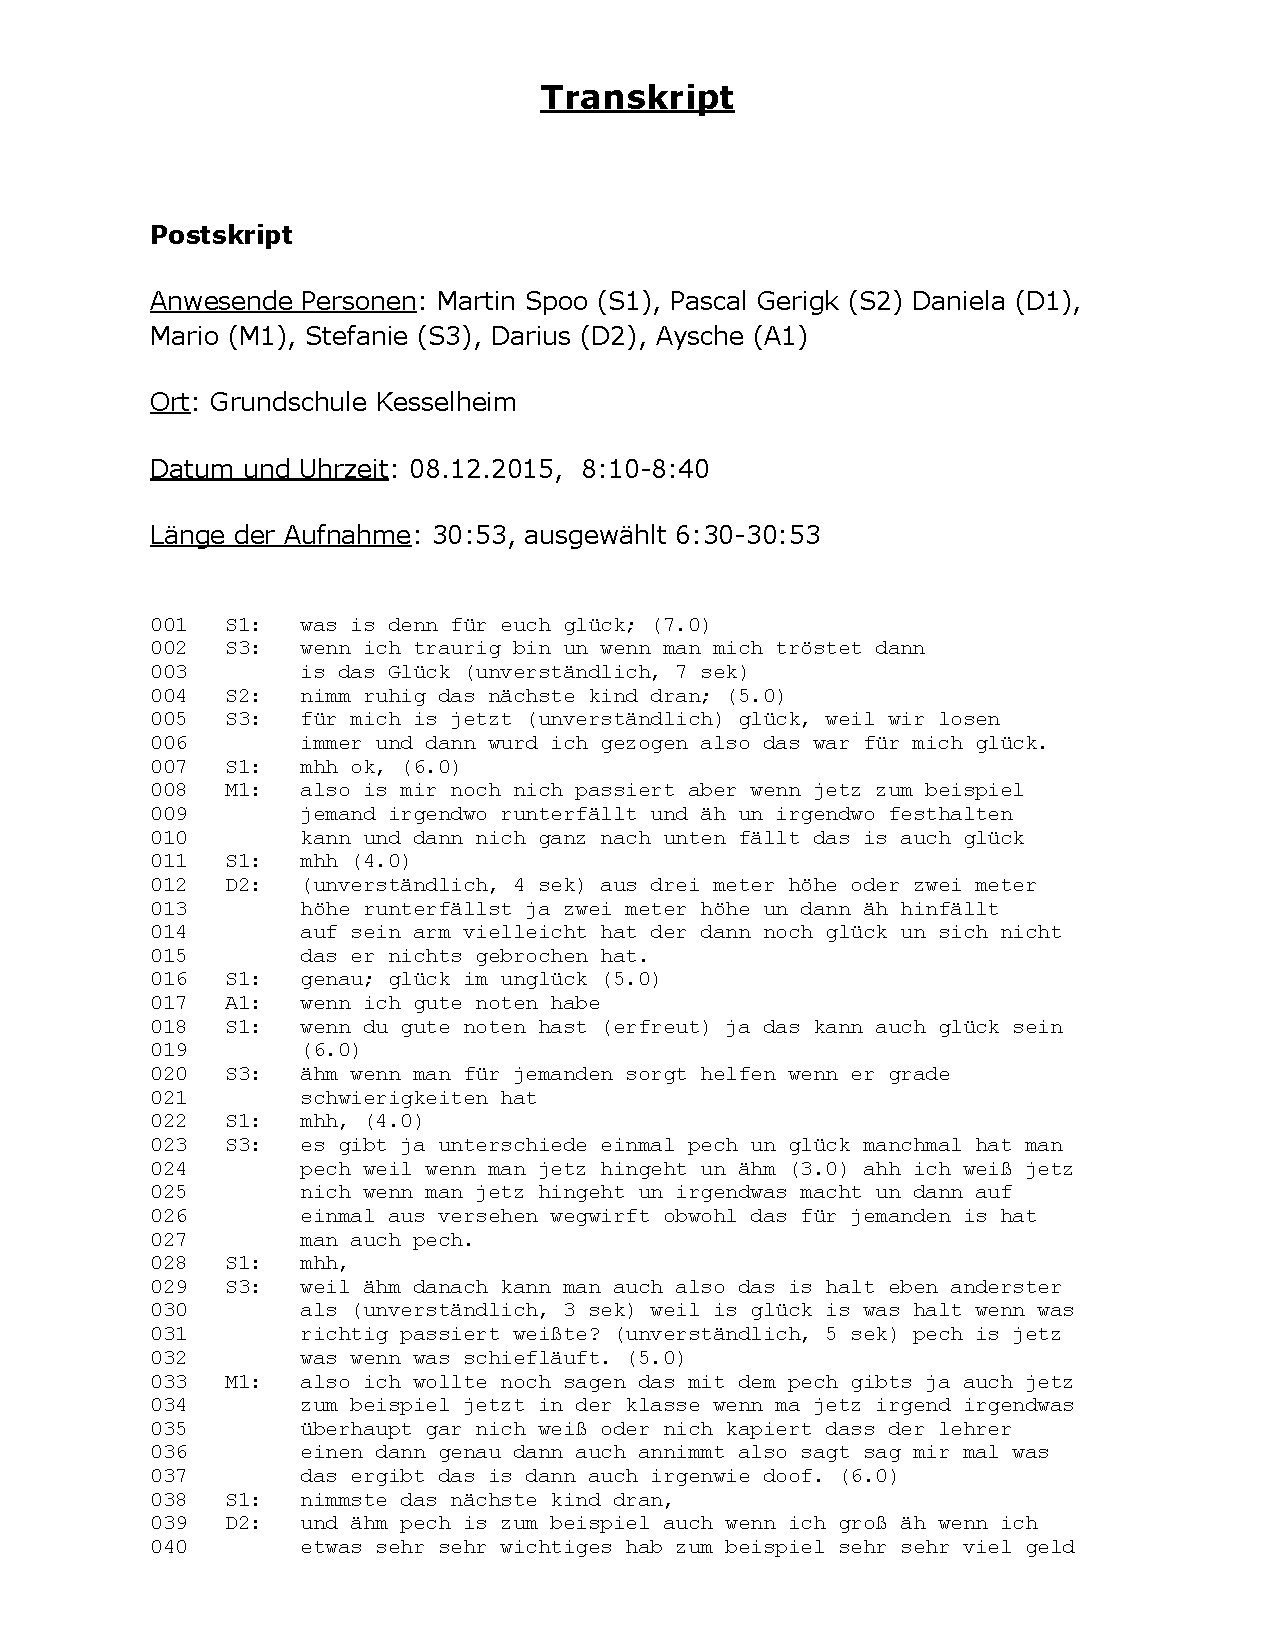
\includepdf[pages={1-6}]{Transkript_Nummern.pdf}
\newpage


\clearpage
%\bibliography{master_thesis}
%\bibliographystyle{dinat}

\newpage
\newgeometry{left=1.5cm,right=1.5cm,head=1.5cm,bottom=1.5cm}
\currentpdfbookmark{Erklärung}{pdf:declaration}
\thispagestyle{empty}
\vspace*{3cm}
\begin{center}
	\Large{\textbf{Erklärung}}
\end{center}
\vspace*{1cm}
Hiermit bestätige ich, dass die vorliegende Arbeit von mir selbstständig verfasst wurde und ich keine anderen als die angegebenen Hilfsmittel - insbesondere keine im Quellenverzeichnis nicht benannten Internet-Quellen - benutzt habe und die Arbeit von mir vorher nicht in einem anderen Prüfungsverfahren eingereicht wurde.
Die eingereichte schriftliche Fassung entspricht der auf dem elektronischen Speichermedium. (CD-ROM)
\vspace*{1cm}\\
Koblenz, den \today
\vspace*{0.75cm}\\
Martin Spoo
\restoregeometry


\end{document}

